\chapter{Introduction}
\label{sec:introduction}

\section{Overview}
\label{sec:introduction:overview}

In the standard model (SM), the interaction between the weak boson and the leptons is expressed by the Lagrangian term $\bar{\chi}_L \gamma^\mu \big( g T_a W^a_\mu +g'Y B_\mu \big) \chi_L + \bar{\psi}_R \gamma^\mu (g' Y B_\mu) \psi_R $, where the coupling constant $g$ is the same for all three lepton generations. Namely,
\begin{equation*}
	g_e = g_\mu = g_\tau \equiv g.
\end{equation*}

\noindent The lepton universality (LU) test in the \PW boson's interaction is an important aspect to test the SM and probe new physics. The LU test has been performed by many particle physics experiments, approaches of which primarily include using the decay of \PW boson produced in the colliders, using the weak decay of mesons, and using the weak decay of leptons. Section~\ref{sec:relatedWorks:lu} in this introduction briefly reviews these activities. Among them, the most related experiments to this thesis are performed with the decay of the \PW bosons produced in the high-energy colliders.


% SPS+Tevatron
The earliest LU test of this kind can be traced back to the SPS experiments, UA1~\cite{Albajar:1988ka} and UA2~\cite{appel1986measurement, Alitti:1991eh, Alitti:1992hv}, at CERN in the 1980s. The measurements were then improved by the Tevatron experiments, CDF~\cite{Abazov:2003sv, Abe:1990sd, Abe:1992ys, Abe:1991fb} and D0~\cite{ Abbott:1999tt, Abachi:1995xc, Abbott:1999pk}, at Fermilab during Tevatron's run-1 from 1985 to 1995. Both SPS and Tevatron produced \PW bosons from the $p\bar{p}$ collisions. One of the common features of these experiments was that the measured quantity was the product of the inclusive \PW cross-section and the \PW leptonic branching fraction, $\sigma_W \times B^W_\ell$, for the three lepton generations. The LU tests were performed by taking the ratios of the measured $\sigma_W \times B^W_\ell$ between two different lepton generations. For \PW coupling to the electron and tau, the combined SPS and Tevatron result~\cite{Abbott:1999pk} showed
\begin{equation*}
    R_{\tau/e} = g^W_\tau / g^W_e = 0.988 \pm 0.025 \qquad \text{(SPS+Tevatron)}.
\end{equation*}
\noindent Overall, the SPS and Tevatron results hinted no clear sign of LU violation related to the \PW boson. 



% LEP
The most precise measurement of the three \PW leptonic branching fractions $B^W_e, B^W_\mu, B^W_\tau$ comes from the four LEP experiments, ALEPH~\cite{Heister:2004wr}, DELPHI~\cite{Abdallah:2003zm}, OPAL~\cite{Abbiendi:2007rs}, L3~\cite{Achard:2004zw} during the LEP's run-2 (1995-2000) which produced $WW$ pairs from the electron-positron collisions. By now, the four LEP experiments are still the only \PW leptonic branching fraction measurements included in the PDG. The experimental precision of $B^W_e, B^W_\mu, B^W_\tau$ has not been improved since LEP. The combined LEP result~\cite{Schael:2013ita} gave $B^W_e = 10.71(16)\%$, $B^W_\mu = 10.63(15)\%$, $B^W_\tau = 11.38(21)\%$. Assuming partial universality for electron and muon, ratio between the tauonic and the average of electronic and muonic branching fraction was reported~\cite{Schael:2013ita} as
\begin{equation*}
    R_{\tau/(e,\mu)} = \frac{2\times B^W_\tau }{B^W_e +  B^W_\mu} = 1.066 \pm 0.025 \qquad \text{(LEP)}.
\end{equation*}

\noindent In comparison, the SM predictions~\cite{Denner:1991kt,Rtau,dEnterria:2016rbf} for $R_{\tau/(e,\mu)}$ is 0.99912,  
%is $R_{\tau/e} \equiv B^W_\tau/B^W_e = 0.99912$ and $R_{\mu/e} \equiv B^W_\mu/B^W_e = 1.00000$ 
taking into account the electromagnetic radiation correction and effect of the lepton mass in the \PW decay phase space. LEP's $R_{\tau/(e,\mu)}$ shows a 2.6 standard deviation ~\cite{Schael:2013ita} from the SM prediction. This moderate deviation motivates the measurement of the branching fractions more precisely.





% LHC
The opportunities arrive in the LHC era. During the LHC run-2, proton and proton collision at $\sqrt{s}=13~\TeV$ allows an unprecedentedly large cross-section for the top quark pair production and produces a large number of \ttbar events. Since the top quark decays almost exclusively into the \PW boson and the $b$ quark, with the help of the improved b-tagging techniques \cite{Chatrchyan:2012jua, Sirunyan:2017ezt, Bols:2020bkb}, it is possible to select a large and pure sample of \ttbar events with two \PW bosons, which can then be used to study \PW boson decays. A recent measurement by the ATLAS collaboration~\cite{Aad:2020ayz} has exploited such a strategy to measure the $R_{\tau/\mu}=B^W_\tau/B^W_\mu$ ratio by fitting the impact parameter distribution of the final state muons. The resulting value is $R_{\tau/\mu} = 0.992 \pm 0.013$, suggesting that lepton universality is preferred. 


% CMS
In the CMS, there has been a significant improvement on the identification of the hadronic tau leptons \cite{Chatrchyan:2012zz, Khachatryan:2015dfa, Sirunyan:2018pgf}, which further opens the door to efficiently select \ttbar events with the $\tau_h$ final state in addition to electron and muon final state, and therefore to measure all the three leptonic branching fractions simultaneously. The CMS analysis in this thesis is performed under this context ---

% \begin{itemize}
%     \item Motivations:
%         \begin{itemize}
%             \item Measurement of $B^W_e, B^W_\mu ,B^W_\tau$ has not been improved for more than a decay since LEP.
%             \item $2.6~\sigma$ deviation between LEP's $R_{\tau/(e,\mu)}$ and the SM requires additional measurement.
%         \end{itemize}
    
%     \item Opportunity:
%         \begin{itemize}
%             \item $\sqrt{s}=13~\TeV$ p-p collision at the LHC produces an increased number of \ttbar events which give $WW$ pairs.
%             \item Improved b-tagging allows to select \ttbar events with a high purity.
%             \item Improved $\tau_h$ identification allows more efficient selection involving $\tau_h$ final state.
%         \end{itemize}
% \end{itemize}


    \noindent \textbf{Motivations:}
        \begin{itemize}
            \item $B^W_e, B^W_\mu ,B^W_\tau$ measurements have not been improved for more than a decay since LEP;
            \item $2.6~\sigma$ deviation between LEP's $R_{\tau/(e,\mu)}$ and the SM appeals additional measurements.
        \end{itemize}
    
    \noindent \textbf{Opportunities:}
        \begin{itemize}
            \item $\sqrt{s}=13~\TeV$ p-p collision at the LHC produces an increased number of \ttbar events which give $WW$ pairs;
            \item the improved b-tagging allows to select \ttbar events with a high purity;
            \item the improved $\tau_h$ identification enables to efficiently select \ttbar events with $\tau_h$ final state in addition to electron and muon final state.
        \end{itemize}

    
    


We have performed a simultaneous measurement of $B^W_e, B^W_\mu ,B^W_\tau$ and the inclusive hadronic branching $B^W_h$. $35.9~\fbinv$ of data collected by the CMS at $\sqrt{s} =13~\TeV$ during the 2016 run of the LHC are analyzed by selecting events consistent with the decay of \ttbar and $tW$. The final states resulting from either one or both of the \PW bosons decaying leptonically are considered.  To collect these events, single electron and single muon triggers are used, thus requiring that the final state must contain at least one prompt electron or muon. Based on the final state objects, data sample are split into a few channels including $e e, \mu\mu,  e\mu, e \tau_h, \mu\tau_h, e\text{+jets}, \mu\text{+jets}$. The estimation of the W branching fractions is carried out based on two separately-developed approaches: 

\begin{table}[!htbp]
    \centering
    \setlength{\tabcolsep}{0.5 em}
    \renewcommand{\arraystretch}{2}
    \begin{tabular}{ >{\centering}m{0.22\textwidth}|m{0.7\textwidth} }
        \hline
        \textbf{Shape analysis}      & template fit the \pt distribution of the sensitive leptons in different channels. \\ 
        \hline
        \textbf{Counting analysis}   & construct ratios of yields for channels with the same trigger and analytically solve three leptonic branching fractions from a set of quadratic equations. \\ 
        \hline
    \end{tabular}
\end{table}


The shape analysis is designed to push forward the precision beyond LEP. It makes the most advantage of the shape information of the lepton \pt spectrum to discriminate the electron and muon coming from $W\to e/\mu$ and from $W\to\tau \to e/\mu$. Comparing with the lepton impact parameter, \pt can be calibrated more conveniently using the energy correction provided the CMS physics object group (POG), and systematics uncertainty associated with the \pt is also expected to be smaller. To achieve better precision, shape analysis includes extra orthogonal regions besides the \ttbar enriched regions, thus constraining some of the most offending systematics such as those related to $\tau_h$ reconstruction. 

The counting analysis is designed to cross-check the shape analysis, with more emphasis on the robustness over precision. It eliminates the shape information and uses only the \ttbar concentrated regions. By constructing the ratios of yields for channels with the same trigger, it has the benefit of canceling some systematics uncertainties related to \ttbar cross section, trigger efficiency and luminosity, and being robust with the lepton energy calibration. However, its precision is highly bottlenecked by the tau identification systematics, ultimately being less sensitive than the shape analysis. 

This thesis describes both the approaches and their results. For $B^W_\tau$, the shape analysis achieves an absolute uncertainty of $2.1\%$, while the uncertainty of counting analysis about $6.7\%$. The final result of shape and counting analysis agree with each other within 1 sigma. In the CMS publication, the more precise result from the shape analysis is reported as the official CMS result to the physics community, and to be compared to and combined with the LEP, while briefly mentioning the cross-check from the counting analysis. 

With the simultaneously measured $B^W_e, B^W_\mu ,B^W_\tau$ and their correlation, the pair-wised ratios between two branching fractions are calculated to test the SM LU prediction. Furthermore, the leptonic and inclusive hadronic branching fraction under the lepton universality assumption are also estimated by repeating the shape analysis with the same parameter for three leptonic branching fractions. From the measured $B^W_\ell$ or $B^W_h$, some SM quantities can be derived, as listed in Table~\ref{tab:introduction:derivedQuantity}. With the SM CKM unitarity, the strong coupling constant $\alpha_s(m_W)$ can be calculated; alternatively, using the latest experimental measurement of $\alpha_s(m_W)$, the square sum of the six CKM elements in the first two rows can be calculated and compared with the unitarity. Among the six elements in the square sum $\sum_{\substack{uc\\dsb}} |V_{ij}|^2$, $V_{cs}$ has the least experimental precision, currently at percent level. So we can take a step further to determine $V_{cs}$ using the experimental values of five other CKM elements. The mathematics and physics related to these derivations are covered in Section~\ref{sec:relatedWorks:vcs}.


% The result of CMS simultaneous measurement of the three W leptonic branching fractions are


% \begin{equation*}
%     B^W_e=10.83(10)\%, ~ B^W_\mu=10.94(08)\%, ~ B^W_\tau=10.77(21)\% \qquad \text{(CMS)}.
% \end{equation*}



% \begin{figure}[!htbp]
%     \centering
%     % 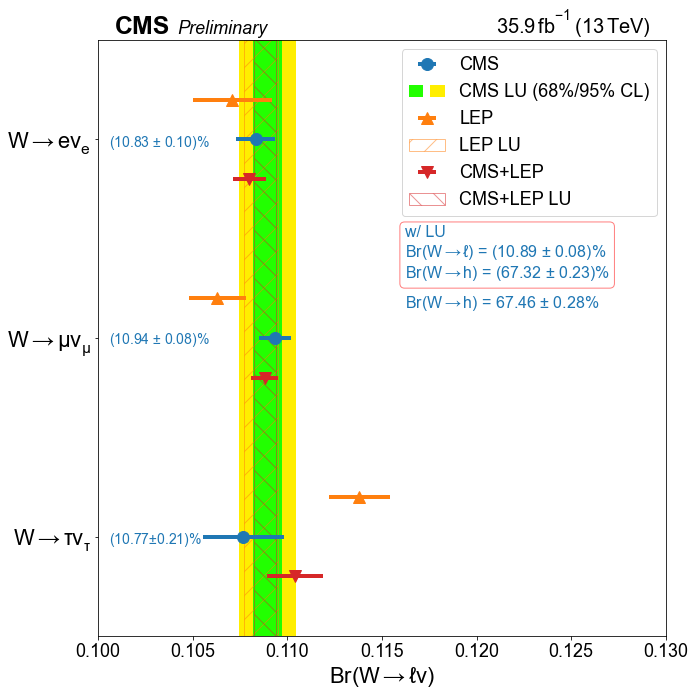
\includegraphics[width=0.5\textwidth]{chapters/Introduction/figures/cms1d.png}
%     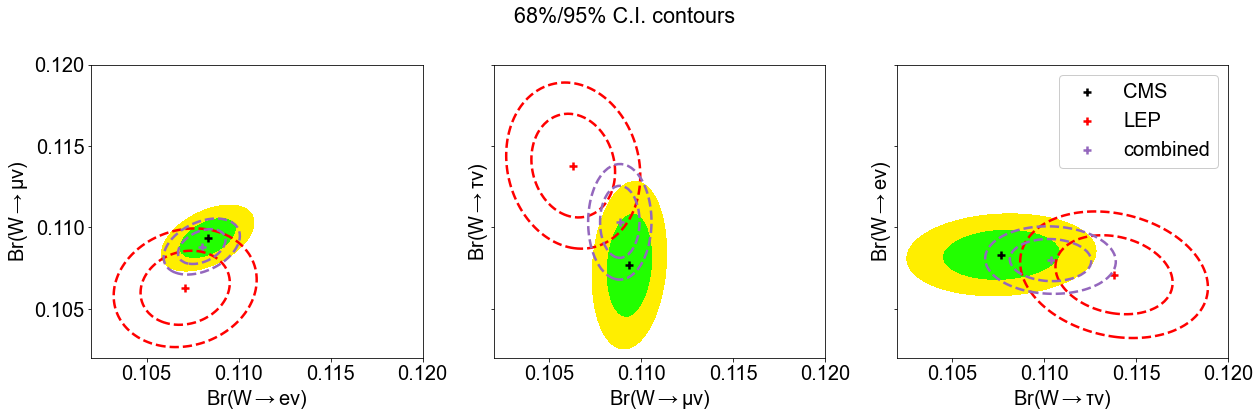
\includegraphics[width=0.99\textwidth]{chapters/Introduction/figures/image.png}
%     \caption{Our simultaneous measurement of the three W leptonic branching fraction with the CMS experiment. }
%     \label{fig:introduction:cmsMoneyPlot}
% \end{figure}


% \noindent Figure~\ref{fig:introduction:cmsMoneyPlot} illustrates the CMS result on the 2D plane of pairs of leptonic branching fraction, together with the comparison and combine with the LEP result. Our result indicates no clear LU violation. If assuming LU, we get $B^W_l=10.89(08)\%, ~ B^W_h=67.32(23)\%$. Comparing with the LEP result, the CMS precision is about 1.6x (2.0x) better on the electronic (muonic) \PW branching fraction, while achieving the same precision on the tauonic one. Combining the CMS with LEP, the world average of $B^W_e,B^W_\mu,B^W_\tau$ measurement is significantly improved, which is the first time for more than a decade since LEP. 


% Based on the measured inclusive hadronic branching fraction $B^W_h$ under the LU hypothesis, some other related SM quantities can be derived. The thory related to the derivation is shown in Section. The full result of the derived quantity is presented in Section. Assuming 

\begin{table}[!h]
    \setlength{\tabcolsep}{0.5em}
    \renewcommand{\arraystretch}{1.5}
    \centering
    \caption{SM quantities can be derived from the measured $B^W_\ell$ or $B^W_h$. }
    \resizebox{0.92\textwidth}{!}{
    \begin{tabular}{ccc}
        % \hline
        Assumption &  & Derived quantity \\
        \hline
        CKM Unitarity $\sum_{uc,dsb} |V_{ij}|^2 = 2$ & $\Longrightarrow$ & $\alpha_s(m_W)$  \\%= 0.094\pm0.033$
        \hline
        PDG $\alpha_s(m_W) = 1.1120\pm0.010$~\cite{pdg2020}     & $\Longrightarrow$ & $\sum_{\substack{uc\\dsb}} |V_{ij}|^2 $ \\ %= 1.985\pm0.021
        \hline
        PDG $\alpha_s(m_W) = 1.1120\pm0.010$~\cite{pdg2020}    & \multirow{2}{*}{$\Longrightarrow$} & \multirow{2}{*}{$V_{cs}$}  \\ %= 0.968\pm 0.011
        PDG $|V_{ud}|^2 + |V_{us}|^2 +|V_{ub}|^2 +|V_{cd}|^2 +|V_{cb}|^2=1.0490(18)$~\cite{pdg2020} & &\\
        \hline
    \end{tabular}}
    \label{tab:introduction:derivedQuantity}
\end{table}




For the outlook of this measurement in the LHC run~3 and High Luminosity LHC (HL-LHC)~\cite{Apollinari:2284929} runs, the further precision improvement can be contributed from the advancement of the $\tau_h$ identification, as well as the improvement of the impact parameter resolution if it is included as additional discriminating observables in the future. In the era of HL-LHC, a few exciting upgrades of the CMS detector will have been accomplished after the phase-2 upgrade~\cite{CMSCollaboration:2015zni}. A new tracker system~\cite{Klein:2017nke} will improve the resolution of the impact parameter. A new endcap calorimeter, the high granularity calorimeter (HGCAL)~\cite{Collaboration:2293646}, is expected to improve the $\tau_h$ identification by allowing novel deep learning algorithms based on its high-resolution jet images. This thesis also describes a new clustering algorithm developed for HGCAL reconstruction and the corresponding high-performance computing using GPUs.



The rest of this introduction chapter covers brief reviews of the related LU tests and $V_{cs}$ measurements. 
Chapter 2 and 3 describe the related SM/BSM physics and the key aspects of the CMS experiment, respectively.
Chapter 4 presents the method and the result of the measurement of the \PW branching fractions, followed by the supplement studies in Chapter 5.
Chapter 6 shows the clustering algorithm developed for the HGCAL reconstruction and its high performance computing using GPUs.















% A fundamental test of lepton universality in the electroweak sector is to measure the branching fractions of the W boson.  The most precise measurements of these quantities were measured at LEP~\cite{Schael:2013ita} and the results of all four experiments are combined to form the world averages~\cite{Patrignani:2016xqp}.  The values measured at each experiment and their combined values are shown in figure~\ref{fig:introduction:wbr}.

% \begin{figure}[ht]
%     \centering
%     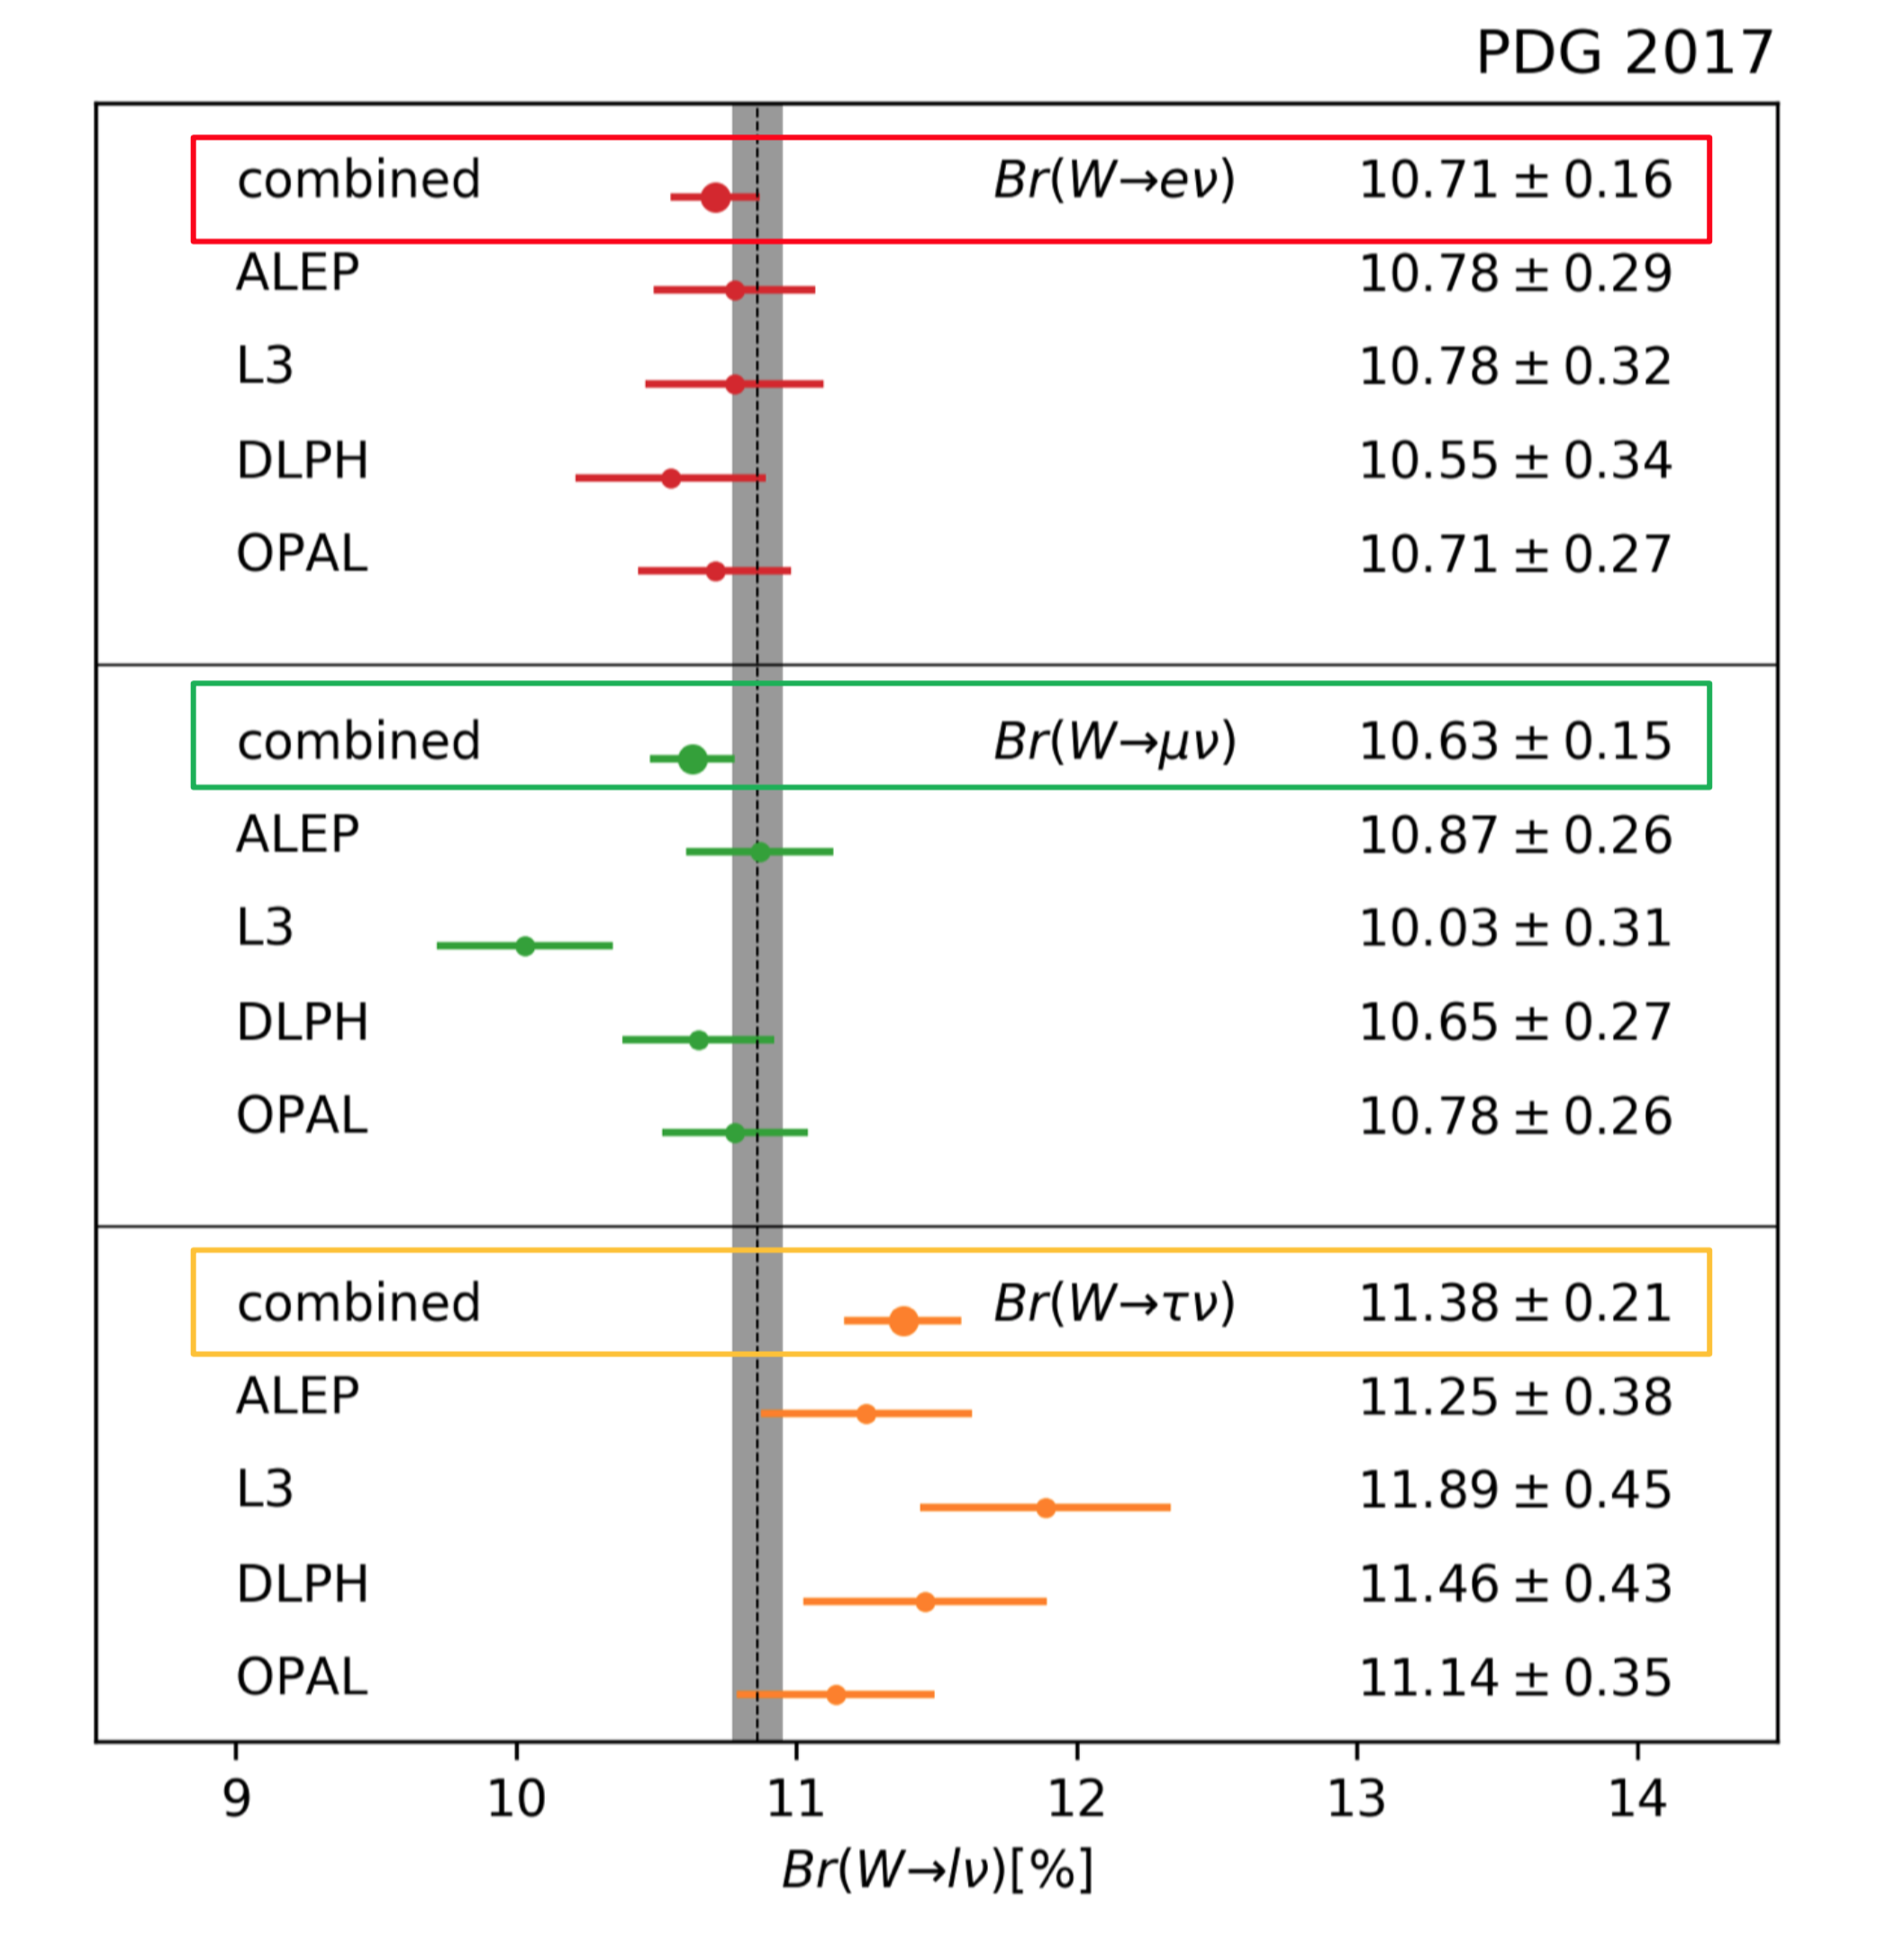
\includegraphics[width=0.6\textwidth]{chapters/Introduction/figures/wdecay.png}
%     \caption{Measured leptonic and inclusive hadronic W branching fractions from LEP.}
%     \label{fig:introduction:wbr}
% \end{figure}


% These measurements show a $\sim 2.6~\sigma$ difference between the tau branching fraction in the case that the fit is carried out assuming lepton universality and the case that each of the branching fractions can vary independently.  This motivates measuring the branching fractions more precisely.  Because of the large number of \ttbar events produced at the LHC, it is possible to select a high statistics, high purity dataset containing two W boson decays which can be used to precisely measure the W branching fractions.  


% In this analysis, $35.9\fbinv$ of data collected by CMS at $\sqrt{s} =13$ TeV during the 2016 run of the LHC are analyzed by selecting events consistent with the decay of pair-produced top quarks or W bosons are selected.  Final states resulting from either one or both of the W bosons decaying leptonically are considered.  To collect these events, single lepton triggers are used thus requiring that the final state must contain at least one prompt electron or muon. 

% Estimation of the values of the W branching fractions is carried out based on two approaches: 

% \begin{itemize}
%     \item maximum likelihood estimation (MLE), binning the data based on the number of b-tags and channel-dependent kinematic information. This will be referred to as the \emph{shape analysis}.
%     \item a semi-analytic approach that constructs ratios of yields in the various channels in a manner that mimics a direct construction of the branching fraction.  This approach does not use kinematic shape information, but does divide channels based on the number of b tags. This will be referred to as the \emph{counting analysis}.
% \end{itemize}




% 
\section{Experimental Test of Lepton Universality}
\label{sec:relatedWorks:lu}

The SM lepton universality (LU) when interacting with W boson is encoded in the Lagrangian term $\bar{\chi}_L \gamma^\mu \big( i \partial_\mu -g \frac{\tau_a}{2} W^a_\mu -g'\frac{Y}{2} B_\mu \big) \chi_L $ in Equation~\ref{eqn:relatedWorks:qft:gws:lagragian}, where the coupling constant $g$ is the same for all three leptons. Namely,
\begin{equation}
	g_e^W = g_\mu^W = g_\tau^W \equiv g
\end{equation}
Precision measurement of the couplings to the weak force of the three leptons provides an excellent test of the lepton universality and the SM. And deviation from the of lepton universality could indicate new physics beyond the standard model. Some of the BSMs allowing non-universality observations are discussed in Section~\ref{sec:relatedWorks:bsm}. So far, the precision test of LU in the weak sector has been performed in a wide variety of particle physics experiments, including but not limited to experiments at the $p\bar{p}, e^+ e^-, pp$ colliders, meson factories, and tau factories. The most related to this thesis are in the colliders using the decay of on-shell W bosons produced in the collision, including SPS, Tevatron, LEP, and LHC experiments. This section summarizes the tests with on-shell W bosons in the colliders, followed by a brief discussion about the LU test using the weak decay in the precision meson physics and tau physics. Among the tests, there are two most well-known anomalies, the LEP results and the semileptonic decay of B mesons, which are also discussed in this section. 


\subsection{Test with on-shell W Decay}
\label{sec:relatedWorks:lu:W}


The on-shell W bosons can be produced on the  $p\bar{p}, e^+ e^-, pp$ colliders. The measurement of the leptonic decay of the on-shell W boson provides one of the most direct LU tests of $g^W_l$. Until 2020, the history of the LU test with on-shell W bosons can be divided into three stages:

\begin{itemize}
    \item CERN SPS (1981-1991) and Fermilab Tevatron (Run-I 1985-1995) using $p \bar{p} \to W + X$.
    \item CERN LEP (Run-II 1995-2000) using $e^+e^- \to W^+  W^-$.
    \item CERN LHC since 2011. W are produced via many processes, but the major processes for the published measurements include $pp \to W +X$ (Run-I) and $pp \to t \bar{t} \to Wb+Wb$ (Run-II)
\end{itemize}

The earliest test can be traced back to the SPS experiments at CERN in the 1980s. Then the measurement was improved by the Tevatron experiments at Fermilab during the Run-I 1985-1995. Both the collider produced W bosons from the $p\bar{p}$ collisions. The key feature of the result in the first stage was that the measured quantity was $\sigma_W \times B(W\to l\nu)$ instead of the three individual $B(W\to l\nu)$, because $W$ boson was just discovered, and its production cross-section $\sigma_W$ was not known well enough. The second era was marked by the LEP experiments, which gave the latest and most precise test before this thesis. One of the key features of the LEP result was that the three leptonic branching fractions were measured simultaneously, together with the corresponding 3x3 correlation matrix. The combined result of LEP experiments showed a 2.6 $\sigma$ deviation from SM lepton universality. This observation is one of the major motivations of the tests in the LHC era, such as this analysis.


\subsubsection{SPS and Tevatron Experiments}



% SPS Tevatron result plot
\begin{figure}[ht]
    \centering
    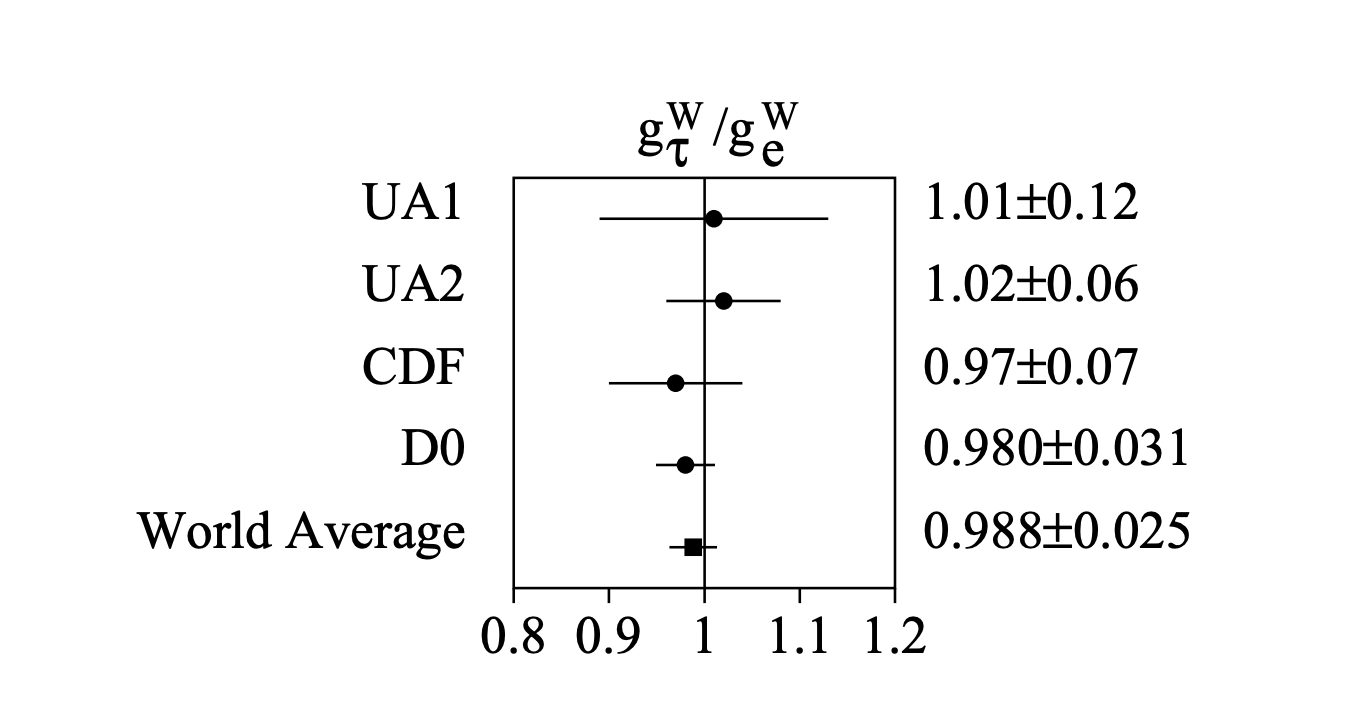
\includegraphics[width=0.5\textwidth]{chapters/RelatedWorks/sectionLU/figures/spsTevatron.png}
    \caption{ $g^W_\tau / g^W_e$ measured in the SPS and Tevatron experiments \cite{Abbott:1999pk}. In all the four experiments, the lepton universality between electron and tau, concerning the weak coupling to W boson, is observed and is consistent with the SM prediction $g^W_\tau / g^W_e=1$ within one experimental uncertainty. The SPS+Tevatron combined result confirms the lepton universality with precision at 2.5\% relative uncertainty on $g^W_\tau / g^W_e$. }
    \label{fig:relatedWorks:lu:W:spsTevatronCombinedRatio}
\end{figure}

The UA1, UA2 experiment at the CERN SPS and CDF, D0 experiment at the Fermilab Tevatron have measured the $p\bar{p} \to W + X$ production cross-section in the three leptonic channels, the ratios of which provides a test of lepton universality concerning the couplings to the on-shell W boson. Figure~\ref{sec:relatedWorks:lu:W:spsTevatron} shows the measurement of $\sigma_W \times B(W\to l \nu)$ in the SPS and Tevatron experiments.  Figure~\ref{fig:relatedWorks:lu:W:spsTevatronCombinedRatio} from \cite{Abbott:1999pk} summarizes the results of $g^W_\tau / g^W_e$ measurements in the SPS and Tevatron experiments. All four measurements confirm consistency with the SM lepton universality within one experimental uncertainty. The combined average is calculated by D0 in \cite{Abbott:1999pk}, the latest published result among the four. In the combining, the systematics in different experiments are assumed to be uncorrelated. The combined result is also consistent with the lepton universality with a precision level at 2.5\%, which can be translated into a precision level of about  5\% on the W branching ratio $B(W\to \tau) / B(W\to e)$.

Both SPS and Tevatron collide protons and anti-protons. SPS operated at CERN from 1981 to 1991 at a center-of-mass energy of 0.546 TeV and 0. 630 TeV. The SM electroweak bosons, W and Z, were first discovered on the SPS in 1983. In 1985, Tevatron at Fermilab began operations at a higher center-of-mass energy at 1.8 TeV, which was later upgraded to 1.96 TeV in the second run since 2001. Tevatron was in service for more than 20 years until 2010 to give ways to the LHC. Based on the discovery and studies of weak bosons on the SPS, Tevatron experiments continued on more precise measurements of the properties of the W and Z bosons. Here lists the key results from the SPS and Tevatron experiments  related to the lepton universality test.



% and had two major experiments UA1 and UA2, which discovered the electroweak bosons W and Z predicted by the GWS EW theory in 1983. The collision energy of SPS was later surpassed by Tevatron at Fermilab in 1986. Since then Tevatron operated more than 20 years until 2010 to give ways to LHC. The two major experiments at Tevatron are D0 and CDF which measured the properties of W and Z boson with improved precision. With respect to testing the lepton universality in the W sector, the SPS and Tevatron experiments share many similarities. They did not directly measured the three leptonic decay branching fractions of W, mainly because the W cross section was not measured precisely at their experimental period. Instead, they measured the cross section of W production in the three leptonic channel. Namely, the product of the W+X produciton cross section and three leptonic W decay branching fractions. 
% UA1 and UA2 experiments in the SPS performed the early measurement of W production cross section in the three leptonic decay channels of W boson. 

UA1 was a general-purpose particle detector at the CERN SPS, consisting of the inner tracker, ECAL HCAL, and a muon system, sequentially from the inside to the outside.  It took 0.546 TeV and 0.63 TeV data during 1982-1983 and 1984-1985, respectively. Its result of W boson studies was summarized in \cite{Albajar:1988ka}. $W \to e \nu$ events were selected based on single-electron plus met selection. The QCD and $W\to \tau_e \nu$ background were estimated with data-driven and MC approach, respectively. In total, 59 and 240 $W \to e \nu$ events were selected from the 0.546 TeV and 0.63 TeV collision, respectively.  $W \to \mu \nu$ events were selected based on single muon plus met selection. The background involving muons from tau and meson decays was estimated by proper simulations. In total, 10 and 57 $W\to \mu\nu$ events were selected from the 0.546 TeV and 0.63 TeV data.  $W\to \tau \nu$ were selected with a single hadronic tau plus met selection. The hadronic taus are identified by highly collimated narrow jets with low charged-track multiplicity.  A $\tau$-likelihood is calculated for jet candidates based on the their shape and charged tracks. In total, 32 events were selected from the combined 0.546 TeV and 0.63 TeV dataset. Based on the yields, UA1 reports the $\sigma_W \times Br(W\to l\nu) $ for the three leptons $l=e,\mu,\tau$ at 0.546 TeV and 0.63 TeV center-of-mass energy. Pair-wise ratios of  $\sigma_W \times Br(W\to l\nu) $ were calculated to test the lepton universality. Table~\ref{tab:relatedWorks:lu:W:sps} lists the $\sigma_W \times Br(W\to l\nu) $ and ratios from UA1.



UA2 was a particle detector at the CERN SPS, consisting of a tracking system surrounded by a calorimetry system with EM and hadronic compartments. Unlike UA1, UA2 is not a multipurpose detector; its focus was on the calorimeters and did not have a muon detector. Therefore, lepton universality test on UA2 mainly involved the $W \to e\nu$ and $W \to \tau \nu$. \cite{appel1986measurement} summarized the $\sigma_W \times Br(W\to e \nu) $ measurements on UA2 using 0.546 TeV and 0.63 TeV data collected during 1982-1983 and 1984-1985. The measurement is based on single-electron plus met trigger. This  $\sigma_W \times Br(W\to e \nu) $ result is shown in Table~\ref{tab:relatedWorks:lu:W:sps}. After the UA2 upgrade during 1985-1987,  the tau channel was added and a test of the lepton universality between $\tau$ and $e$ was performed \cite{Alitti:1991eh, Alitti:1992hv}, using the 0.63 TeV data collected during 1988-1990. The hadronic taus were reconstructed from jet candidates with selections on relative hadronic energy and the lateral energy profile. The data is triggered with the met trigger in 1988-1989 and hadronic tau trigger in 1990. \cite{Alitti:1991eh} analyzed the 1988-1989 data, while \cite{Alitti:1992hv} combined the 1988-1989 data with 1990 data. The result \cite{Alitti:1992hv} for the ratio between tauonic and electronic W decays is shown in the Table~\ref{tab:relatedWorks:lu:W:sps}. 

\begin{figure}[ht]
    \centering
    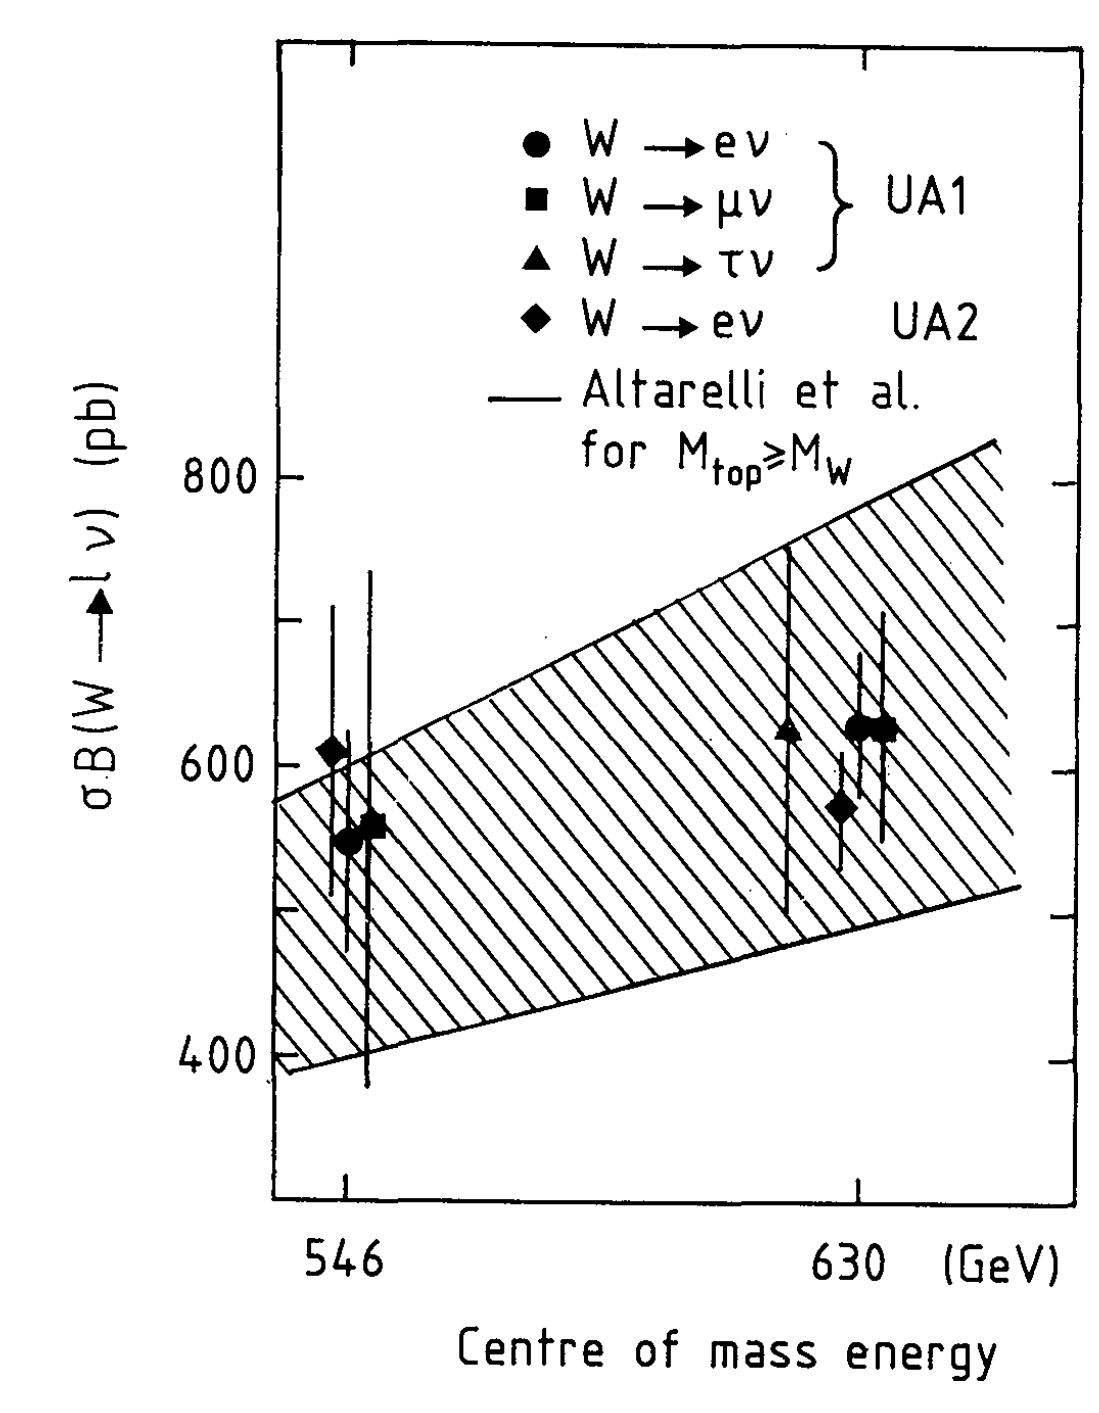
\includegraphics[width=0.35\textwidth]{chapters/RelatedWorks/sectionLU/figures/SPS.png}
    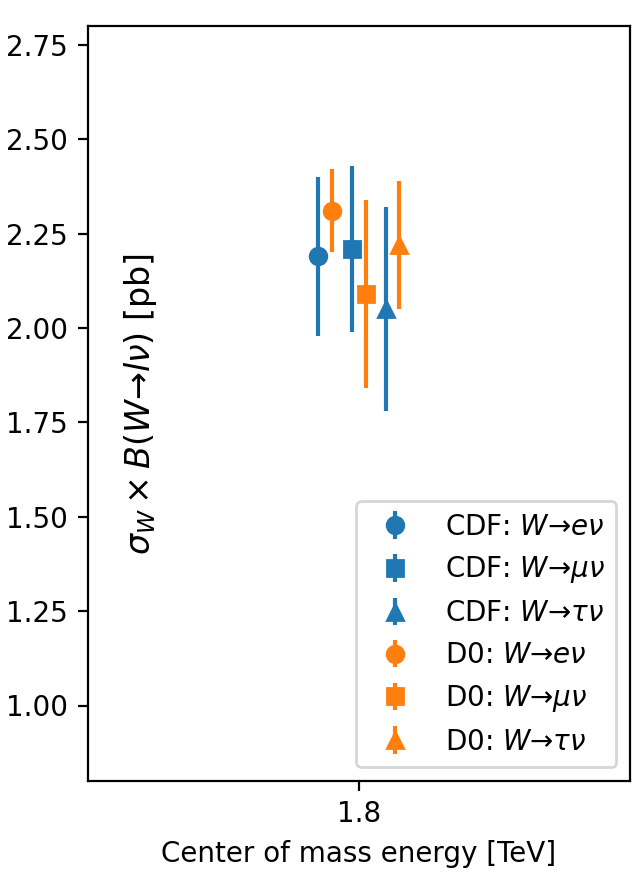
\includegraphics[width=0.6\textwidth]{chapters/RelatedWorks/sectionLU/figures/tevatron.png}
    \caption{Measurement of $\sigma_W \times B(W\to l \nu)$ in the SPS \cite{Albajar:1988ka} and Tevatron experiments. [RIGHT plot needs reproduce] }
    \label{sec:relatedWorks:lu:W:spsTevatron}
\end{figure}

% SPS result table
\begin{table}[ht]
    \setlength{\tabcolsep}{ 0.5 em}
    \renewcommand{\arraystretch}{1.5}
    \centering
    \caption{The measurement of $\sigma_W \times B(W\to l \nu)$ and the ratios between leptonic channels in the UA1 and UA2 experiment at the CERN SPS. }
    \resizebox{\textwidth}{!}{
    \begin{tabular}{ |c|l l| } 
         
         % UA1 result
         \hline
         \multicolumn{3}{|c|}{UA1 \cite{Albajar:1988ka} }  \\
         \hline
         & $p\bar{p}$ at $\sqrt{s}=0.546$ TeV &  $p\bar{p}$ at $\sqrt{s}=0.630$ TeV \\
         \hline
         $\sigma_W \times Br(W\to e    \nu)$  [nb]  & 0.55 $\pm$ 0.08 (stat) $\pm$ 0.09 (syst) & 0.63 $\pm$ 0.06 (stat) $\pm$ 0.10 (syst) \\ 
         $\sigma_W \times Br(W\to \mu  \nu)$  [nb]  & 0.56 $\pm$ 0.18 (stat) $\pm$ 0.12 (syst) & 0.63 $\pm$ 0.08 (stat) $\pm$ 0.11 (syst) \\ 
         $\sigma_W \times Br(W\to \tau \nu)$  [nb]  & \multicolumn{2}{c|}{ 0.63 $\pm$ 0.13 (stat) $\pm$ 0.12 (syst) }  \\ 
         \hline
         $Br(W\to \mu  \nu)/ Br(W\to e \nu)$  & \multicolumn{2}{c|}{1.00  $\pm$ 0.14 (stat) $\pm$ 0.08 (syst) } \\
         $Br(W\to \tau \nu)/ Br(W\to e \nu)$  & \multicolumn{2}{c|}{1.02  $\pm$ 0.20 (stat) $\pm$ 0.10 (syst) } \\
         
         \hline
         \multicolumn{2}{c}{} \\
         
         % UA2 result
         \hline
         \multicolumn{3}{|c|}{UA2}  \\
         \hline
         & $p\bar{p}$ at $\sqrt{s}=0.546$ TeV &  $p\bar{p}$ at $\sqrt{s}=0.630$ TeV \\
         \hline
         $\sigma_W \times Br(W\to e    \nu)$  [nb] \cite{appel1986measurement} & 0.50 $\pm$ 0.09 (stat) $\pm$ 0.05 (syst) & 0.53 $\pm$ 0.06 (stat) $\pm$ 0.05 (syst) \\ 
         % This is UA2 result reported in the UA1 summary
        %  $\sigma_W \times Br(W\to e    \nu)$  [nb] \cite{Albajar:1988ka} & 0.61 $\pm$ 0.10 (stat) $\pm$ 0.07 (syst) & 0.57 $\pm$ 0.04 (stat) $\pm$ 0.07 (syst) \\ 
         \hline
         $Br(W\to \tau \nu)/ Br(W\to e \nu)$ \cite{Alitti:1992hv} & - & 1.04  $\pm$ 0.08 (stat) $\pm$ 0.08 (syst) \\
         
         \hline
    \end{tabular}}
    \label{tab:relatedWorks:lu:W:sps}
\end{table}




% Tevatron result table
\begin{table}[ht]
    \setlength{\tabcolsep}{0.5 em}
    \renewcommand{\arraystretch}{1.5}
    \centering
    \caption{The measurement of $\sigma_W \times B(W\to l \nu)$ and the ratios between leptonic channels in the CDF and D0 experiment at the Fermilab Tevatron.}
    \resizebox{\textwidth}{!}{
    \begin{tabular}{ |c|l| } 
         
         % D0 result
         \hline
         \multicolumn{2}{|c|}{D0 with $p\bar{p}$ at $\sqrt{s}=1.8$ TeV} \\
         \hline
         $\sigma_W \times Br(W\to e    \nu)$  [nb] \cite{Abbott:1999tt} & 2.31 $\pm$ 0.01 (stat) $\pm$ 0.05 (syst) $\pm$ 0.10 (lum) \\ 
         $\sigma_W \times Br(W\to \mu  \nu)$  [nb] \cite{Abachi:1995xc} & 2.09 $\pm$ 0.23 (stat) $\pm$ 0.11 (syst) \\ 
         $\sigma_W \times Br(W\to \tau \nu)$  [nb] \cite{Abbott:1999pk} & 2.22 $\pm$ 0.09 (stat) $\pm$ 0.10 (syst) $\pm$ 0.10 (lum)  \\ 
         \hline
         $Br(W\to \mu  \nu)/ Br(W\to e \nu)$ \cite{Abachi:1995xc} & 0.89  $\pm$ 0.10 \\
         $Br(W\to \tau \nu)/ Br(W\to e \nu)$ \cite{Abbott:1999pk} & 0.961 $\pm$ 0.061 \\
         
         \hline
         \multicolumn{2}{c}{} \\
         
         
         %  CDF result
         \hline
         \multicolumn{2}{|c|}{CDF with $p\bar{p}$ at $\sqrt{s}=1.8$ TeV} \\
         \hline
         $\sigma_W \times Br(W\to e    \nu)$  [nb] \cite{Abe:1990sd}    & 2.19 $\pm$ 0.04 (stat) $\pm$ 0.21 (syst) \\ 
         $\sigma_W \times Br(W\to \mu  \nu)$  [nb] \cite{Abe:1992ys}    & 2.21 $\pm$ 0.07 (stat) $\pm$ 0.21 (syst) \\ 
         $\sigma_W \times Br(W\to \tau \nu)$  [nb] \cite{Abe:1991fb}    & 2.05 $\pm$ 0.27 \\ 
         \hline
         $Br(W\to \mu  \nu)/ Br(W\to e \nu)$ \cite{Abe:1992ys} & 1.02  $\pm$ 0.08 \\
         $Br(W\to \tau \nu)/ Br(W\to e \nu)$ \cite{Abe:1991fb} & 0.94  $\pm$ 0.14 \\

         \hline
    \end{tabular}}
    \label{tab:relatedWorks:lu:W:tevatron}
\end{table}



CDF is an azimuthally and forward-backward symmetric general-purpose detector at the Fermilab Tevatron. It is consists of several subdetector layers, including a silicon tracker, gas chamber as the central outer tracker, solenoid magnet, ECAL/HCAL, and muon detector. CDF began taking its first data in 1985 and started Run I after its first upgrade in 1989. For $W \to e  \nu$, \cite{Abe:1990sd} presents a measurement of $\sigma_W \times B(W\to e \nu)$ using the single-electron trigger with a selection of single isolated electron plus met. For $W \to \mu  \nu$, \cite{Abe:1992ys} presents a measurement of $\sigma_W \times B(W\to \mu \nu)$ and the ratio of muon and electron channel. This measurement used the single-muon trigger with a selection of single isolated muon plus met. Citing the previous CDF result on $\sigma_W \times B(W\to e \nu)$ in \cite{Abe:1990sd}, it obtained the ratio of the muonic and electronic weak coupling as $\frac{g^W_\mu}{g^W_e}=1.01\pm0.04$, consistent with the lepton universality. For $W \to \tau \nu$, \cite{Abe:1991fb} measured the $\sigma_W \times B(W\to \tau \nu)$ and its ratio to the electronic channel previous obtained in the \cite{Abe:1990sd}. The tau channel was based on two triggers, a met trigger and a single-tau trigger, which yielded 132 and 47 final events after selections. Comparing with the met trigger, the tau trigger required an additional tau jet cluster with a lower met threshold. The tau identification required 0-3 tracks with no tracks in the 10\degree - 30 \degree region separate from the seeding track. Combining the met triggered and tau triggered data, the ratio between tau channel and electron channel was reported as $g^W_\tau/g^W_e=0.97\pm0.07$  agreeing with the SM lepton universality, as shown in Figure~\ref{fig:relatedWorks:lu:W:spsTevatronCombinedRatio}. Table~\ref{tab:relatedWorks:lu:W:tevatron} lists the CDF's results about the three $\sigma_W \times B(W\to l \nu)$ and the pair-wise ratios.





D0 was a general-purpose particle detector at the Fermilab Tevatron. Its structure was similar to CDF, consisting of a hybrid tracking system with silicon inner tracker and scintillator fiber outer tracker, superconducting solenoid, ECAL/HCAL, and the muon system. The detector was completed in 1991 and was placed in the Tevatron in February 1992. D0 collected its 1.8 TeV collision data during 1992-1995. With data collected in 1992-1993, D0 presented a measurement of $\sigma_W \times B(W\to e\nu)$, $\sigma_W \times B(W\to \mu \nu)$ and their ratio \cite{Abachi:1995xc}. Later, in the year 1994-1995, about 6 times more data was collected, and accordingly $\sigma_W \times B(W\to e\nu)$ was updated with better precision \cite{Abbott:1999tt}. It is worth noticing that this update \cite{Abbott:1999tt} also reported the branching fraction of W decay into electrons separately from the $\sigma_w$, as $B(W\to e\nu)=(10.66\pm0.15\pm0.21\pm0.11\pm0.11)\%$, where the uncertainties were for statistics, systematics, theory, and NLO. Also, with the 1994-1995 data, D0 measured $\sigma_W \times B(W\to \tau \nu)$ and test the lepton universality between tau and electron \cite{Abbott:1999pk}, shown in Figure ~\ref{fig:relatedWorks:lu:W:spsTevatronCombinedRatio}. For $W \to e \nu$ and $W \to \mu \nu$, the measurement selected events based on single-electron plus met and single-muon plus met. For $W \to \tau \nu$, D0 used a dedicated hadronic tau trigger, which included requirements on the met, the leading narrow jet pt, and no jet opposite to the leading narrow jet. The hadronic taus were reconstructed as boosted narrow jets with cuts on the $E_T$ and the jet width (energy weighted tower size in the jet). For each jet candidate, the energy in the leading two towers over the total energy was used to discriminate the tau jets over the background QCD jets. Table~\ref{tab:relatedWorks:lu:W:tevatron} lists the D0's results about the three $\sigma_W \times B(W\to l \nu)$ and the pair-wise ratios.









% this result is indirect calculation using the LEP inputs
% \cite{Abazov:2003sv} summaries the W mass and witdh measurement on Tevatron by D0 and CDF and reports a tevatron combined W to electron branching fraction as 
% \begin{equation}
%     B(W\to e\nu)=(10.61 \pm 0.28) \% \; \text{Tevatron}
% \end{equation}


\subsubsection{LEP Experiments}
The Large Electron-positron collider (LEP) at CERN increased its collision center-of-mass energy from the Z pole (LEP-I 1989-1995) to a maximum of 209 GeV during its second running phase (LEP-II 1995-2000). In some periods in 1995 and 1997, the LEP was operated at center-of-mass energies below the WW resonance at 130.3, 136.3, and 140.2 GeV. The rest run of LEP-II scanned at 10 different energies above the WW resonance ranging in 161.3 - 209 GeV. During the full second run scanning the center-of-mass energy from 130 GeV to 209 GeV, the four LEP experiments ALEPH, DELPHI, L3, and OPAL, collected a total of 3 $fb^{-1}$ integrated luminosity data. 

The four detectors at LEP were designed to explore the physics at the Z pole during the LEP-I and around WW mass up to 203 GeV during the LEP-II. ALEPH is a cylindrical symmetric detector. It had a tracking system  (drift chamber and TPC) and ECAL inside a supper conducting solenoid. Outside the solenoid were streamer tubes inserted in the iron return yokes for the hadron and muon detection. DELPHI is also a cylindrical general-purpose detector consisting of the vertex detector, TPC tracker, Ring-Imaging Cherenkov detector, ECAL, solenoid, HCAL, muon chamber. OPAL's subdetector layers were formed by vertex detector, tracker, magnetic solenoid, crystal ECAL/HCAL, and muon detector. Unlike the other 3 detectors, L3 had its magnetic solenoid as the outmost layer; inside were trackers (silicon strip micro vertex detector and time expansion chamber), ECAL, HCAL, and muon chamber. 

The WW production in the LEP was mainly induced by the EW process in the t-channel exchanging $\nu_e$, and the triple gauge boson coupling process in the s-channel mediated by Z or photon. The measurement of WW production cross-section combining the four LEP experiments is shown in Figure. There is a clear turn on the WW production above 161.3 GeV. The combined experimental result was consistent with the theoretic prediction from YFSWW ad RACOONWW.

\begin{figure}[ht]
    \centering
    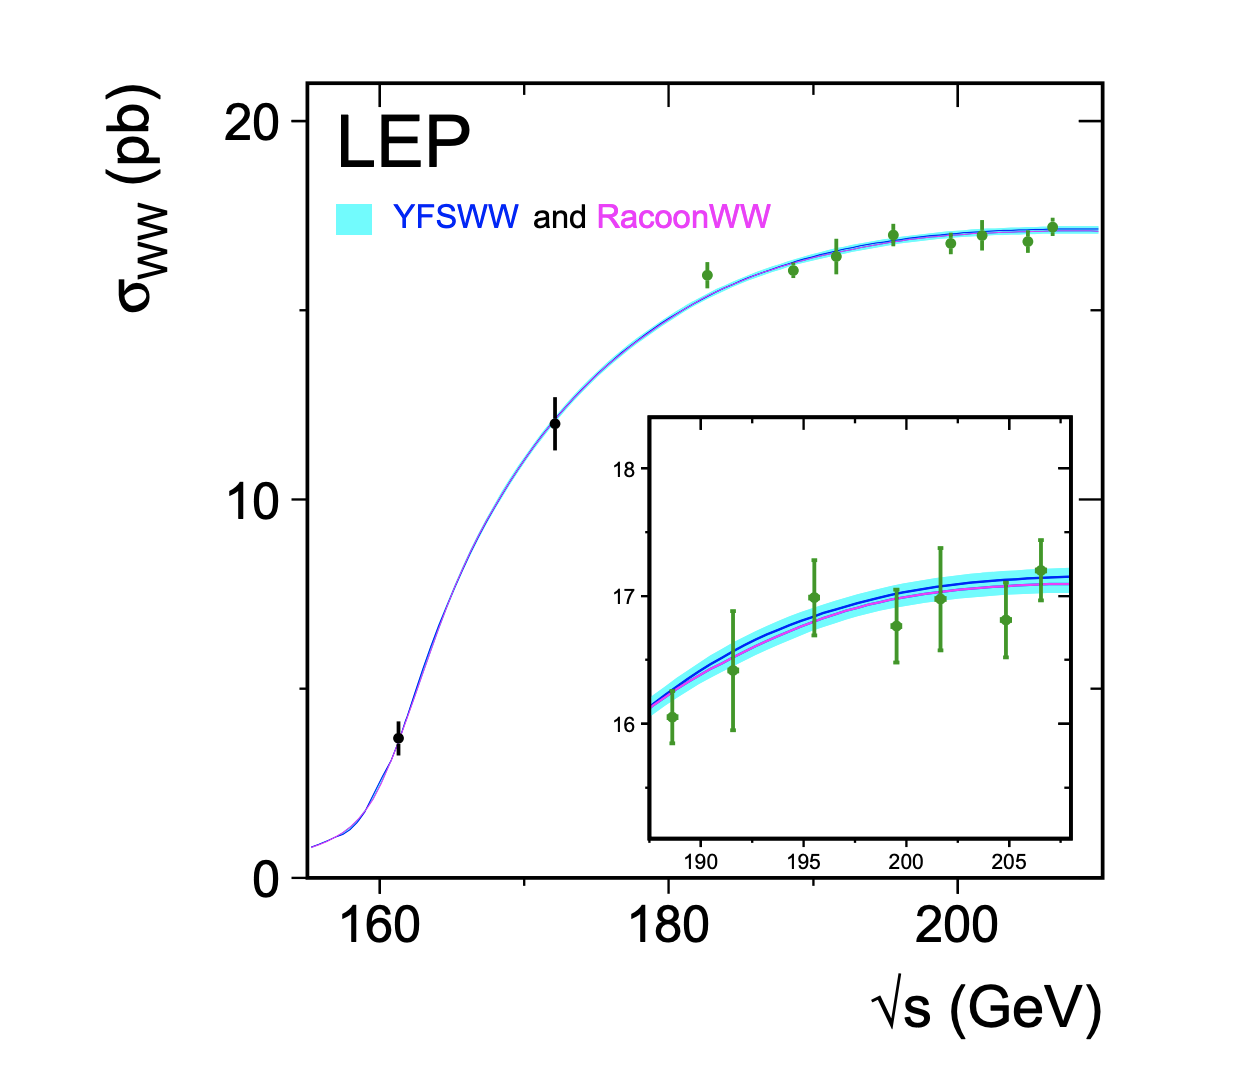
\includegraphics[width=0.49\textwidth]{chapters/RelatedWorks/sectionLU/figures/lep_ww.png}
    \caption{The LEP measurement of WW production cross-section. The measurement was a combine of the four LEP experiments, with a total 3 $fb^{-1}$  data. The WW production at LEP is mainly induced by exchanging neutrinos in the t-channel and quark annihilation to $Z/\gamma$  in the s-channel. The measured cross-section agrees with the theoretical calculation.}
    \label{fig:my_label}
\end{figure}

Each experiment determined the leptonic W branching fractions from the cross-sections of the individual WW decay channels, with and without the lepton universality assumption \cite{Schael:2013ita}. The hadronic branching fraction was determined from the leptonic ones based on the unity summation constraint. When combining the four experiments, the theoretical uncertainties on signal and background, as well as the theoretical uncertainties on the luminosity, were treated correlated; in contrast, the experimental uncertainties on the luminosity, detector effects, and MC statistics are treated uncorrelated. The details of the $B(W\to l \nu)$ results and the 3x3 correlation matrices, in all four experiments and after combined, are summarized in Table~\ref{tab:relatedWorks:lu:W:lep} and in Figure~\ref{fig:relatedWorks:lu:W:lep} . A clear excess of the lepton universality was observed in the result. While the branching fractions to electron and muon agree well with each other, the branching fraction to tau is more than $2 \sigma$ larger than the average of the branching fraction to electron and muon. Assuming only partial lepton universality, the ratio between the $B(W\to \tau \nu)$ and the average of $B(W\to e \nu)$ and $B(W\to \mu \nu)$ were reported as \cite{Schael:2013ita}



\begin{equation*}
    \frac{2\times Br(W\to \tau \nu)}{Br(W\to e \nu)+ Br(W\to \mu  \nu)} = 1.066 \pm 0.025,
\end{equation*}

\noindent showing a 2.6 standard deviation from the lepton universality.


% LEP result plot
\begin{figure}[ht]
    \centering
    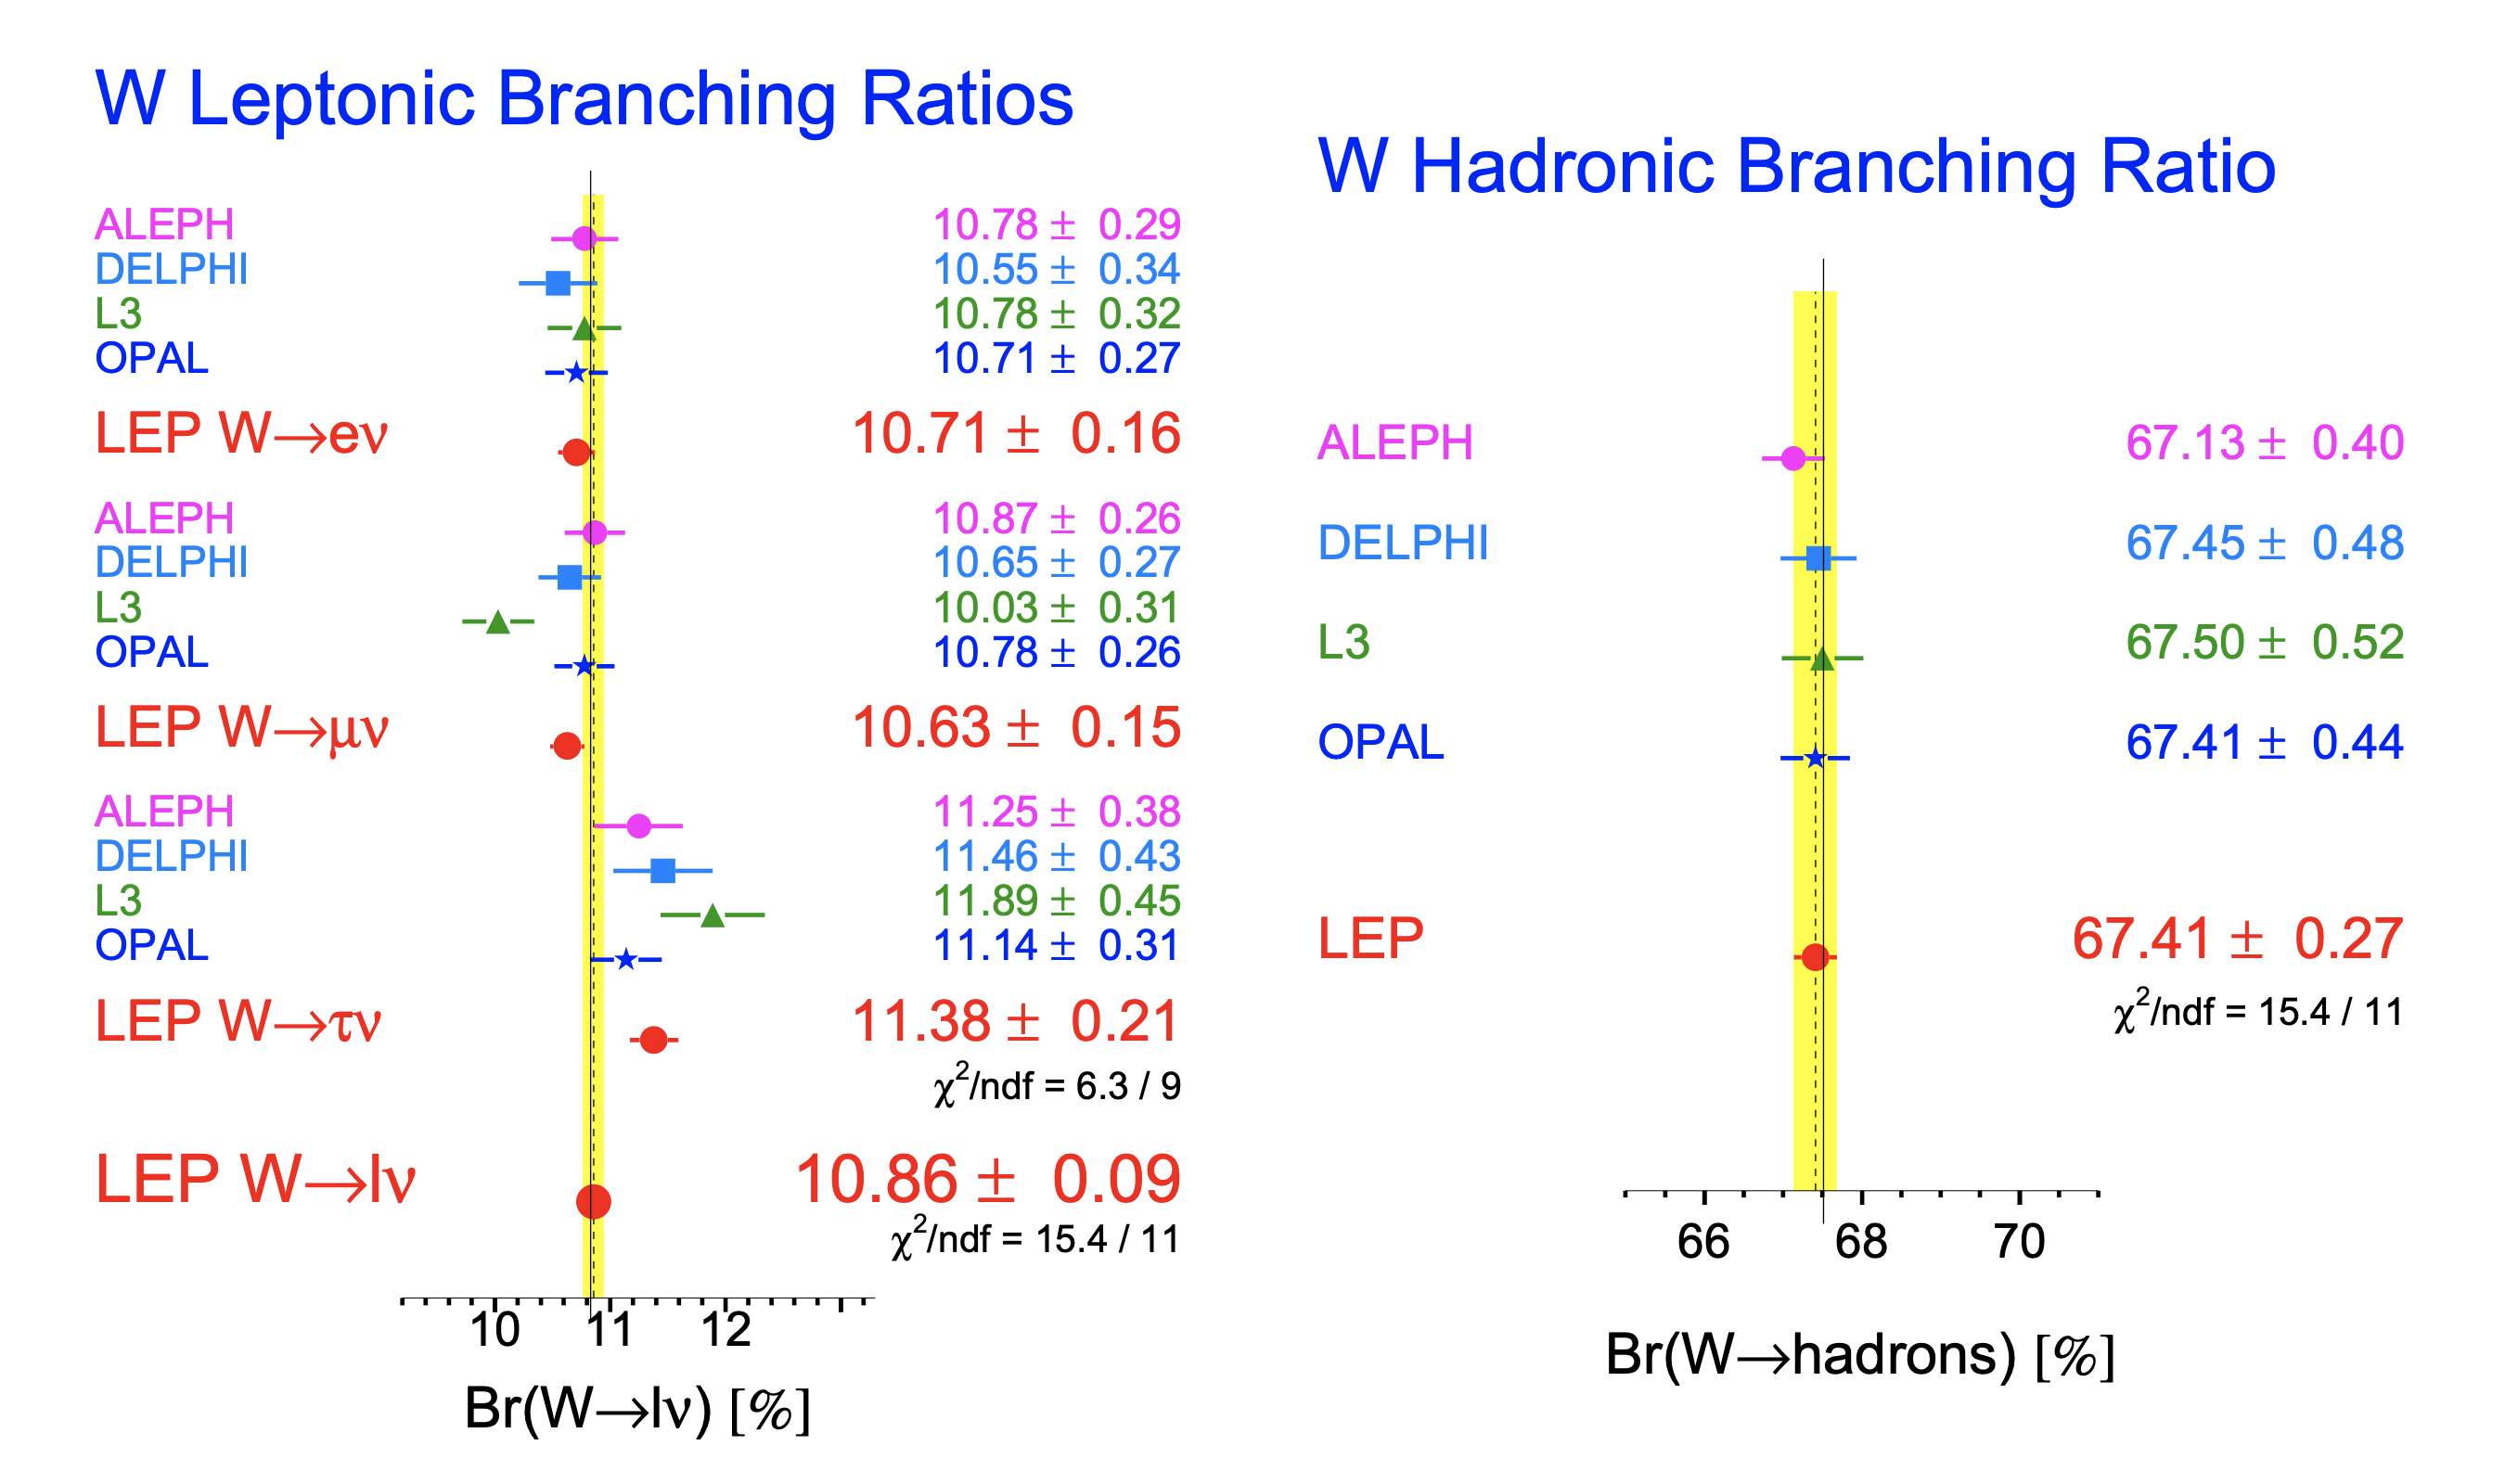
\includegraphics[width=0.99\textwidth]{chapters/RelatedWorks/sectionLU/figures/lepResult.png}
    \caption{Three $B(W\to l \nu)$  and hadronic branching fraction of the four LEP experiments and the combined result. In the LEP average, $B(W\to \tau \nu)$  is 2.6 $\sigma$ larger than the average of $B(W\to e \nu)$ and $B(W\to \mu \nu)$ \cite{Schael:2013ita}. }
    \label{fig:relatedWorks:lu:W:lep}
\end{figure}


% LEP result table
\begin{table}[ht]
    \setlength{\tabcolsep}{.5 em}
    \renewcommand{\arraystretch}{1.5}
    \centering
    \caption{Three $B(W\to l \nu)$ and the 3x3 correlation matrix of the four LEP experiments and the combined result \cite{Schael:2013ita}}
    \resizebox{\textwidth}{!}{
    \begin{tabular}{ |c| c  c | } 
         %  LEP ALEPH
         \hline
         \multicolumn{3}{|c|}{ALEPH \cite{Heister:2004wr}} \\
         \hline
         $Br(W\to e    \nu)$    & 10.78 $\pm$ 0.27 (stat) $\pm$ 0.10 (syst) & 
         \multirow{3}{*}{
            \begin{footnotesize}
            $\begin{bmatrix}
                +1.000 &-0.009 &-0.332 \\ 
                -0.009 &+1.000 &-0.268 \\
                -0.332 &-0.268 &+1.000 
            \end{bmatrix}$ 
            \end{footnotesize} 
         } \\
         $Br(W\to \mu  \nu)$    & 10.87 $\pm$ 0.25 (stat) $\pm$ 0.08 (syst) & \\ 
         $Br(W\to \tau \nu)$    & 11.25 $\pm$ 0.32 (stat) $\pm$ 0.20 (syst) & \\
         \hline
         \multicolumn{3}{c}{} \\
         
         
         %  LEP DELPHI
         \hline
         \multicolumn{3}{|c|}{DELPHI \cite{Abdallah:2003zm}} \\
         \hline
         $Br(W\to e    \nu)$    & 10.55 $\pm$ 0.31 (stat) $\pm$ 0.14 (syst) & 
         \multirow{3}{*}{
            \begin{footnotesize}
            $\begin{bmatrix}
                +1.000 &+0.030 &-0.340 \\ 
                +0.030 &+1.000 &-0.170 \\
                -0.340 &-0.170 &+1.000 
            \end{bmatrix}$ 
            \end{footnotesize} 
         } \\
         $Br(W\to \mu  \nu)$    & 10.65 $\pm$ 0.26 (stat) $\pm$ 0.08 (syst) & \\ 
         $Br(W\to \tau \nu)$    & 11.46 $\pm$ 0.39 (stat) $\pm$ 0.19 (syst) & \\
         \hline
         \multicolumn{3}{c}{} \\
         
         
         %  LEP L3
         \hline
         \multicolumn{3}{|c|}{L3 \cite{Achard:2004zw}} \\
         \hline
         $Br(W\to e    \nu)$    & 10.78 $\pm$ 0.29 (stat) $\pm$ 0.13 (syst) & 
         \multirow{3}{*}{
            \begin{footnotesize}
            $\begin{bmatrix}
                +1.000 &+0.136 &-0.201 \\ 
                +0.136 &+1.000 &-0.122 \\
                -0.201 &-0.122 &+1.000 
            \end{bmatrix}$ 
            \end{footnotesize} 
         } \\
         $Br(W\to \mu  \nu)$    & 10.03 $\pm$ 0.29 (stat) $\pm$ 0.12 (syst) & \\ 
         $Br(W\to \tau \nu)$    & 11.89 $\pm$ 0.40 (stat) $\pm$ 0.20 (syst) & \\
         \hline
         
         \multicolumn{3}{c}{} \\
         
         %  LEP OPAL
         \hline
         \multicolumn{3}{|c|}{OPAL \cite{Abbiendi:2007rs}} \\
         \hline
         $Br(W\to e    \nu)$    & 10.71 $\pm$ 0.25 (stat) $\pm$ 0.11 (syst) & 
         \multirow{3}{*}{
            \begin{footnotesize}
            $\begin{bmatrix}
                +1.000 &+0.135 &-0.303 \\ 
                +0.135 &+1.000 &-0.230 \\
                -0.303 &-0.230 &+1.000 
            \end{bmatrix}$ 
            \end{footnotesize} 
         } \\
         $Br(W\to \mu  \nu)$    & 10.78 $\pm$ 0.24 (stat) $\pm$ 0.10 (syst) & \\ 
         $Br(W\to \tau \nu)$    & 11.14 $\pm$ 0.31 (stat) $\pm$ 0.17 (syst) & \\
         \hline
         
         \multicolumn{3}{c}{} \\
         %  LEP Average
         \hline
         \multicolumn{3}{|c|}{LEP Average \cite{Schael:2013ita}} \\
         \hline
         $Br(W\to e    \nu)$    & 10.71 $\pm$ 0.14 (stat) $\pm$ 0.07 (syst) & 
         \multirow{3}{*}{
            \begin{footnotesize}
            $\begin{bmatrix}
                +1.000 &+0.136 &-0.201 \\ 
                +0.136 &+1.000 &-0.122 \\
                -0.201 &-0.122 &+1.000 
            \end{bmatrix}$ 
            \end{footnotesize} 
         } \\
         $Br(W\to \mu  \nu)$    & 10.63 $\pm$ 0.13 (stat) $\pm$ 0.07 (syst) & \\ 
         $Br(W\to \tau \nu)$    & 11.38 $\pm$ 0.17 (stat) $\pm$ 0.11 (syst) & \\
         \hline
         $Br(W\to \mu  \nu)/ Br(W\to e \nu)$ & 0.993  $\pm$ 0.019 & 
         \multirow{3}{*}{
            \begin{footnotesize}
            $\begin{bmatrix}
                +1.000 &+0.440 &-0.314 \\ 
                +0.440 &+1.000 &+0.714 \\
                -0.314 &+0.714 &+1.000 
            \end{bmatrix}$ 
            \end{footnotesize} 
         } \\
         $Br(W\to \tau \nu)/ Br(W\to e \nu)$ & 1.063  $\pm$ 0.027 & \\
         $Br(W\to \tau \nu)/ Br(W\to\mu\nu)$ & 1.070  $\pm$ 0.026 &  \\
         
         \hline
    \end{tabular}}
    \label{tab:relatedWorks:lu:W:lep}
\end{table}


\subsubsection{LHC Experiments}

During the LHC Run-I at a center-of-mass energy of 7 TeV and 8 TeV, the lepton universality test in the EW sector was studied in the electron and muon channel, taking W+jets events as the signal. Two such measurements were published by the ATLAS and LHCb. ATLAS measured the $\sigma_W \times B(W \to e \nu)$ and $\sigma_W \times B(W \to \mu \nu)$ \cite{Aaboud:2016btc} with 7 TeV proton-proton collision data with 4.6/fb collected in 2011. The events in the electron and muon channel were triggered with the single-lepton trigger and selected with several lepton isolation and identification cut and met cut. The ratio between muon and electron was determined as $\frac{ B(W  \to \mu \nu) }{ B(W \to e \nu)} = 1.003\pm 0.010$. LHCb also measured the $\sigma_W \times B(W \to e \nu)$ \cite{Aaij:2016qqz} and $\sigma_W \times B(W \to \mu \nu)$ \cite{Aaij:2015zlq} in two analysis with 8 TeV LHC data corresponding to 2/fb integrated luminosity. The events were also triggered with the single-lepton, and the selections required on lepton quality and met. To test universality between the electron and muon channel, the second analysis \cite{Aaij:2016qqz} compared the electron channel with the muon channel published in the first analysis \cite{Aaij:2015zlq}, taking into account the experimental correlations. The comparison included both the total cross-section and the differential cross-section with respect to pseudorapidity. The differential cross-section agreed well in the electron and muon channel. The ratio of the two total cross-section led to $\frac{ B(W  \to \mu \nu) }{ B(W \to e \nu)}  = 0.980 \pm 0.018 $




During the LHC Run-II at a unprecedentedly high center-of-mass energy of 13 TeV, for the first time since the SPS era in the 1980s, W bosons from the $t\bar{t}$ events are treated as the major signal in the LU test,  thanks to the high $t\bar{t}$ cross-section at 13 TeV. In addition, compared to the LHC Run-I, the improvement of the hadronic tau reconstruction also allows better precision tests involving the tau channel. This is the context of our analysis. Related to our analysis, ATLAS recently measured the ratio between W to tau and W to muon branching fraction $B(W  \to \tau \nu) / B(W \to \mu \nu) $ using the LHC Run-II data from 2016-2018 at 13 TeV corresponding to 139/fb. The analysis selects tt events with a single-muon trigger and applies additional requirements on muon quality, jet multiplicity, and bTag multiplicity for a tt-concentrated region. The two W bosons from tt decay are used for the analysis (need double check, make sure not one-tag one-prob). Tau is probed with tau's muonic decay, which is 17\% of the total tau decay width. The key technique of this ATLAS measurement is fitting to the vertex displacement of the selected muon to discriminate $W \to \mu$ and $W \to \tau \to \mu$. Probing tau with muonic decay and dividing by the $W \to \mu$ help cancel the systematical uncertainties related to the muon reconstruction. Also, the systematics concerning hadronic tau reconstruction is avoided. The limitation of this approach is that only the $B(W  \to \tau \nu) / B(W \to \mu \nu) $ ratio is measured but the three individual leptonic branching fractions are not. The reported result of the $\tau / \mu $ branching ratio is

$$ \frac{ B(W  \to \tau \nu) }{ B(W \to \mu \nu)}  = 0.992 \pm 0.013 \text{ (ATLAS Run-II) }$$





\subsection{Test with Meson Decay}
\label{sec:relatedWorks:lu:meson}


% meson decay table
\begin{table}[ht]
    \setlength{\tabcolsep}{.5 em}
    \renewcommand{\arraystretch}{1.5}
    \centering
    \caption{SM prediction and the experimental measurements of the leptonic or semi-leptonic branching ratios of the pseudoscalar mesons. \cite{Bifani:2018zmi} }
    \resizebox{\textwidth}{!}{
    \begin{tabular}{|c|c|c|c|}
        \hline
         & SM Prediction & World Average & Included measurements \\
        \hline
        % pi
        $R^\pi_{e/\mu} \; [10^{-4}]$ &  1.2352 $\pm$ 0.0001 \cite{Cirigliano:2007xi} & 1.2327 $\pm$ 0.0023  & 
            \tiny{ TRIUMF \cite{Numao:1992ve, Britton:1992pg}, PiENu \cite{Aguilar-Arevalo:2015cdf}, BGO-OD \cite{Czapek:1993kc}} \\
        % K
        $R^K_{e/\mu} \; [10^{-5}]$ &  2.477  $\pm$ 0.001 \cite{Cirigliano:2007xi} & 2.488  $\pm$ 0.009 & 
            \tiny{NA62 \cite{Lazzeroni:2012cx}, KLOE \cite{Ambrosino:2009aa} }\\
        % D_s
        $R^{D_s}_{\tau/\mu} $ &  9.76 $\pm$ 0.10 \cite{Dobrescu:2008er} & 9.95 $\pm$ 0.61  & 
            \tiny{ HFLAV \cite{Amhis:2016xyh} ave of CLEO, BASIII, BELLE, BABAR} \\
        
        \hline
        % B D
        $R^{B}_{D, \tau/l} $ &  0.299  $\pm$ 0.003  \cite{Bifani:2018zmi} & 0.340  $\pm$ 0.030 & 
            \tiny{BABAR \cite{Lees:2012xj, Lees:2013uzd}, Belle \cite{Huschle:2015rga} }\\
            
        % B D*
        $R^{B}_{D*, \tau/l} $ &  0.258  $\pm$ 0.005 \cite{Bifani:2018zmi} & 0.295  $\pm$ 0.014 & 
            \tiny{BABAR \cite{Lees:2012xj, Lees:2013uzd}, Belle \cite{Huschle:2015rga, Sato:2016svk, Hirose:2016wfn}, LHCb\cite{Aaij:2015yra,Aaij:2017uff, Aaij:2017deq} }\\
            
        \hline
    \end{tabular}}
    \label{tab:relatedWorks:lu:meson:ratio}
\end{table}

The decay of pseudoscalar mesons provides some of the stringent tests of LU. The most stringent constraints come from the study of leptonic decay of the charged pions or kaons, which are helicity suppressed in the SM depending on the mass of the outcoming lepton. Pions and kaons can decay into electrons and muons, but not taus which are heavier than $\pi, K$. The ratio between the electronic and muonic branching fractions $R^\pi_{e/\mu},R^K_{e/\mu}$ are measured and compared with the SM prediction. For D meson, tauonic decay is possible, and the ratio between tauonic and muonic branching fraction $R^D_{\tau/\mu}$ is measured in the charm factories including CLEO, BASIII, Belle, and BaBar. Table~\ref{tab:relatedWorks:lu:meson:ratio} shows these experimental measurements and the comparison to the SM theoretical calculations. The experimental result of purely leptonic decay of light and charm pseudoscalar meson agree well with the theoretical prediction. Additionally, the tests of LU in FCCC can be performed by comparing semileptonic transitions, such as $K\to \pi l\nu$ and $D\to K l\nu$, with different lepton flavors. However, these tests require knowledge of the ratio of the form factors of the scalar and vector meson, f0/f+, with very high accuracy to be competitive with the leptonic decays, where the main hadronic input (meson decay constants) drops out of the LU ratios. 

Anomaly is observed in the semileptonic decay of B meson. $R^{B}_{D^{(*)}, \tau/l}$ is measured in the Belle, BaBar and LHCb, where ratio is defined as the semileptonic branching fraction with tau over with electron and muon. $R^{B}_{D, \tau/l} = \frac{Br(B\to D+\tau \nu)}{Br(B\to D+l \nu)}$ and $R^{B}_{D^*, \tau/l} = \frac{Br(B\to D^*+\tau \nu)}{Br(B\to D^*+l \nu)}$ where $l=e,\mu$ . Figure~\ref{fig:relatedWorks:lu:meson:bMesonDecay} shows this well-known anomaly of lepton universality in the B meson semileptonic decay. The world average of  Belle, BaBar and LHCb is about 4 sigma deviated from the theoretical prediction with SM. The individual value of the ratios are shown in Table~\ref{tab:relatedWorks:lu:meson:ratio}.

% B meson decay plot
\begin{figure}[ht]
    \centering
    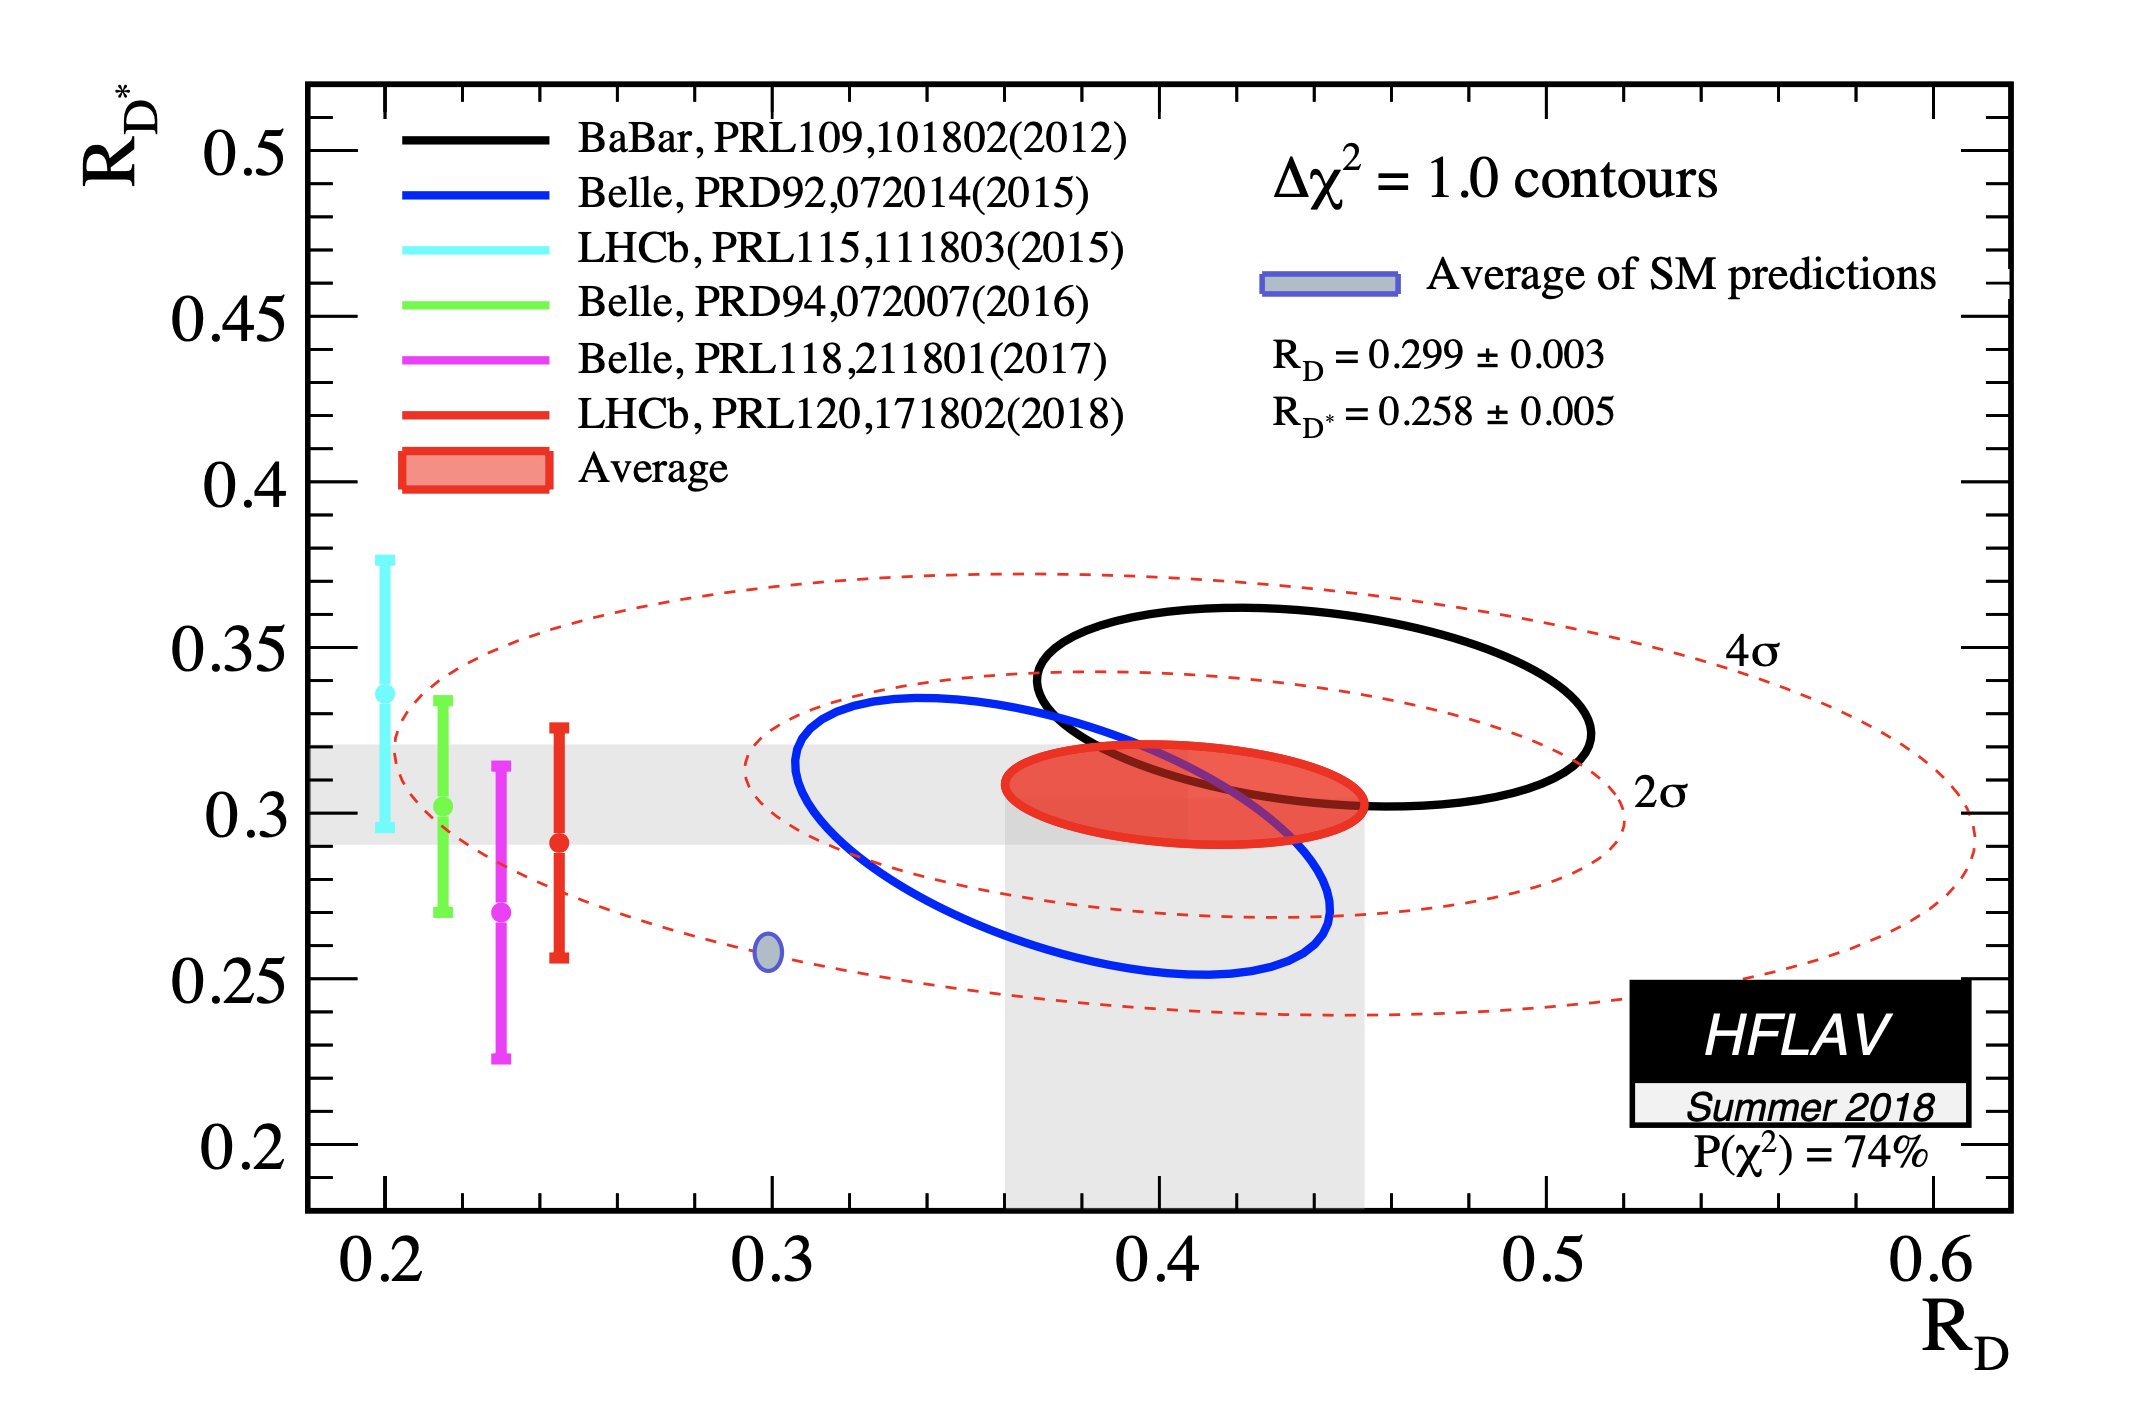
\includegraphics[ width = 0.7 \textwidth ]{chapters/RelatedWorks/sectionLU/figures/bmeson.png}
    \caption{ Anomaly of lepton universality in the semi-leptonic decay of B meson. SM prediction and the world average of $R^{B}_{D, \tau/l}$  and $R^{B}_{D^*, \tau/l}$  shows a 4 sigma deviation.}
    \label{fig:relatedWorks:lu:meson:bMesonDecay}
\end{figure}




\subsection{Test with Tau Decay}
\label{sec:relatedWorks:lu:lepton}

The LU of FCCC transitions can also be tested by the tau precision measurement \cite{Pich:2013lsa}. In the SM, the only expected difference between the $\tau^- \to e^- \bar{\nu}_e \nu_\tau$  and $\tau^- \to \mu^- \bar{\nu}_\mu \nu_\tau$  decay is due to decay kinematic phase space due to the mass difference in the outcoming leptons. $g_\mu  / g_e $ can be obtained by precision measurement of the tau decay in the electron and muon channels. Similarly,  $g_\tau  / g_\mu $ can be obtained by precision measurement of electronic tau decay  $\tau^- \to e^- \bar{\nu}_e \nu_\tau$ and electronic muon decay  $\mu^- \to e^- \bar{\nu}_e \nu_\mu$.  The ratio of the FCCC couplings to the third and first family can be obtained from the measurements of the $\tau^- \to \mu^- \bar{\nu}_\mu \nu_\tau$  and $\mu^- \to e^- \bar{\nu}_e \nu_\mu$  branching fraction and the $\tau,\mu$ lifetimes.  These represent the most stringent experimental tests available today for LU tests in the EW sector. From the tau precision measurement, the ratios of EW coupling constant among the three leptons are \cite{Pich:2013lsa}

\begin{align}
    g_\tau / g_\mu &= 1.0010 \pm 0.0014 \\
    g_\tau / g_e   &= 1.0029 \pm 0.0014 \\
    g_\mu  / g_e   &= 1.0018 \pm 0.0014 
\end{align}






\section{Related Experimental Results}

This section gives a brief review of two sets of related experiments: the LU test in the charged weak sector and the measurements of $V_{cs}$.

\subsection{Test of Lepton Universality of the Charged Weak Current}
\label{sec:relatedWorks:lu}


\subsubsection{Test with \PW Boson Decay} 
\label{sec:relatedWorks:lu:W}

~\\
% Test with \PW boson decay can be summarized into three eras: 1) SPS and Tevatron, 2) LEP, 3) LHC.




% SPS and Tevatron Experiments
\underline{SPS and Tevatron}

Both SPS and Tevatron collide protons and anti-protons. SPS operated at CERN from 1981 to 1991 at a center-of-mass energy of 0.546~\TeV and 0.630~\TeV. The SM electroweak bosons, \PW and \PZ, were first discovered in the SPS in 1983 \cite{ARNISON1983103, BANNER1983476}. In 1985, Tevatron at Fermilab began operations at a higher center-of-mass energy at 1.8~\TeV, which was later upgraded to 1.96~\TeV in its second run since 2001. Tevatron was in service for more than 20 years until 2010 to give ways to the LHC. 
% The properties of the weak bosons were measured with higher precision by Tevatron experiments. 


\begin{figure}[ht]
    \centering
    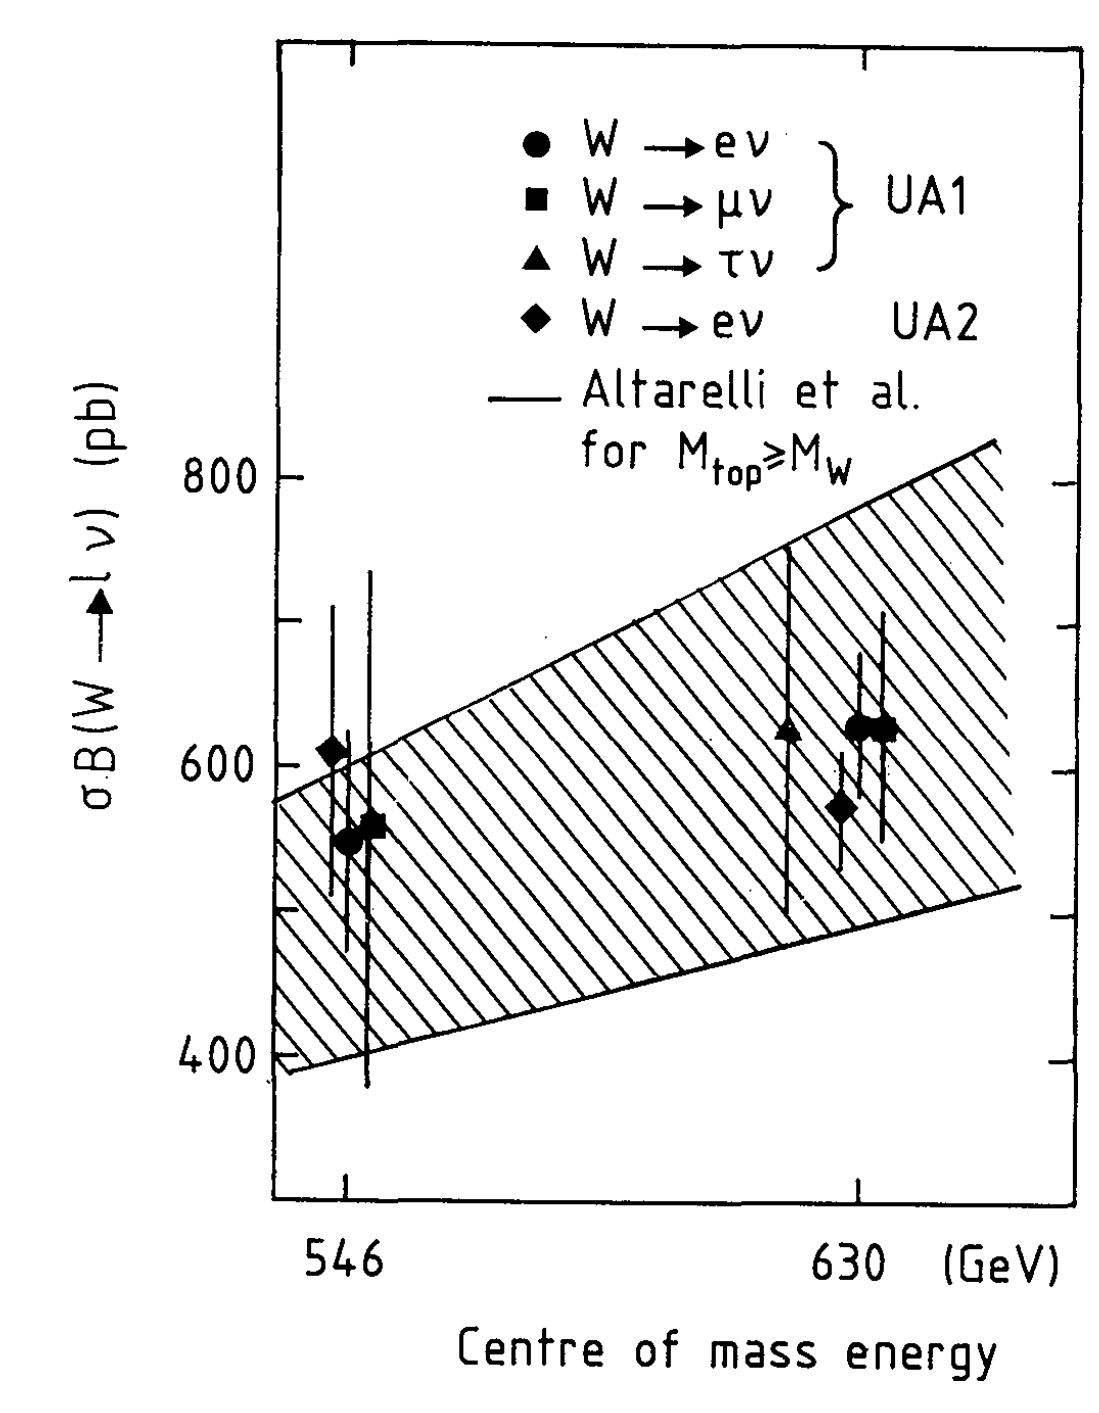
\includegraphics[height=0.35\textheight]{chapters/RelatedWorks/sectionLU/figures/SPS.png} \qquad
    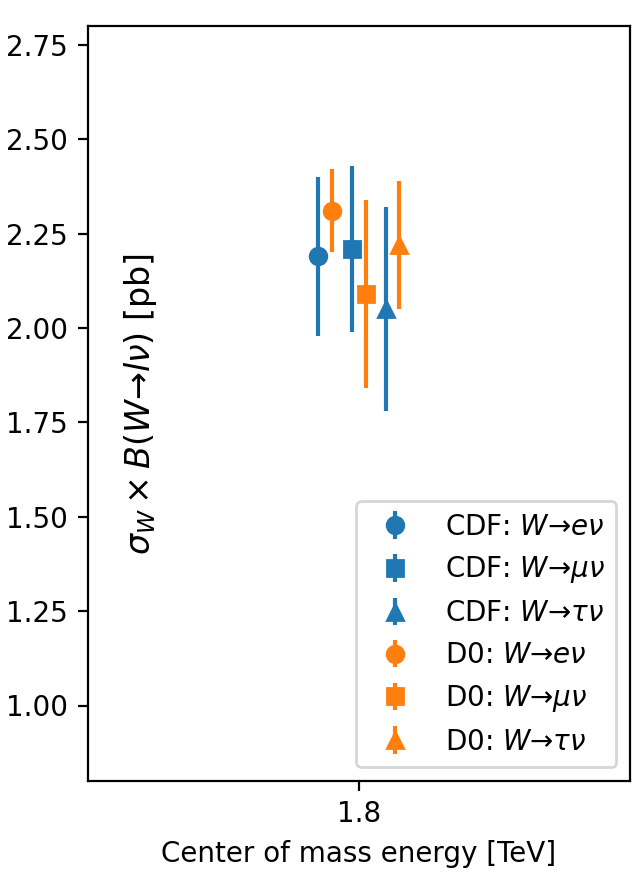
\includegraphics[height=0.35\textheight]{chapters/RelatedWorks/sectionLU/figures/tevatron.png}
    \caption{Measurement of $\sigma_{p\bar{p}\to W} \times B^W_{l \nu}$ by the SPS \cite{Albajar:1988ka} and Tevatron~\cite{Abazov:2003sv, Abbott:1999tt, Abachi:1995xc, Abbott:1999pk, Abe:1990sd, Abe:1992ys, Abe:1991fb} experiments.}
    \label{sec:relatedWorks:lu:W:spsTevatron}
\end{figure}


% SPS Tevatron result plot
\begin{figure}[ht]
    \centering
    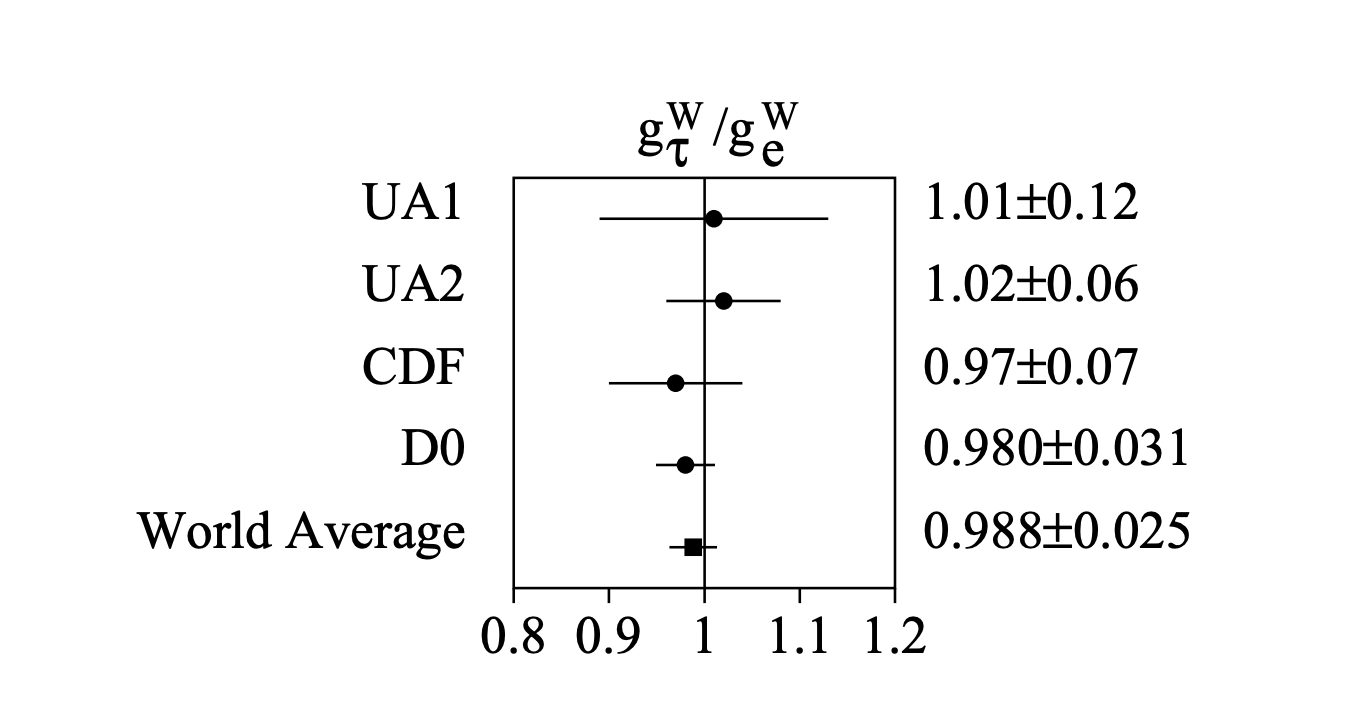
\includegraphics[width=0.5\textwidth]{chapters/RelatedWorks/sectionLU/figures/spsTevatron.png}
    \caption{ $g^W_\tau / g^W_e$ measured in the SPS and Tevatron experiments \cite{Abbott:1999pk}. In all the four experiments, the ratio of the weak coupling constant between electron and tau was extracted by the ratio of $\sigma_{p\bar{p}\to W} \times B^W_{l \nu}$ measurement in the electron and tau channel. The average was combined by D0 collaboration~\cite{Abbott:1999pk}, the last published result among the four.}
    \label{fig:relatedWorks:lu:W:spsTevatronCombinedRatio}
\end{figure}


The UA1, UA2 experiment at the CERN SPS and the CDF, D0 experiment at the Fermilab Tevatron measured the $p\bar{p} \to W \to \ell\nu$ cross-section in the different leptonic channels. Figure~\ref{sec:relatedWorks:lu:W:spsTevatron} shows the measurement of $\sigma_W \times B^W_{l \nu}$ in the SPS and Tevatron experiments. The LU test is performed by taking the ratios of two different leptonic channels. Figure~\ref{fig:relatedWorks:lu:W:spsTevatronCombinedRatio} from \cite{Abbott:1999pk} summarizes the results of $g^W_\tau / g^W_e$ measurements in the SPS and Tevatron experiments. The combined average was calculated by the D0 collaboration~\cite{Abbott:1999pk}, which was the last published result among the four. The combine assumed uncorrelated systematical and statistical uncertainties. And all four measurements confirmed consistency with the SM lepton universality within one experimental uncertainty.







% SPS result table
\begin{table}[ht]
    \setlength{\tabcolsep}{ 0.5 em}
    \renewcommand{\arraystretch}{1.5}
    \centering
    \caption{The measurement of $\sigma_W \times B(W\to l \nu)$ and the ratios between leptonic channels in the UA1 and UA2 experiment at the CERN SPS. }
    \resizebox{\textwidth}{!}{
    \begin{tabular}{ |c|l l| } 
         
         % UA1 result
         \hline
         \multicolumn{3}{|c|}{UA1 \cite{Albajar:1988ka} }  \\
         \hline
         & $p\bar{p}$ at $\sqrt{s}=0.546$ TeV &  $p\bar{p}$ at $\sqrt{s}=0.630$ TeV \\
         \hline
         $\sigma_W \times Br(W\to e    \nu)$  [nb]  & 0.55 $\pm$ 0.08 (stat) $\pm$ 0.09 (syst) & 0.63 $\pm$ 0.06 (stat) $\pm$ 0.10 (syst) \\ 
         $\sigma_W \times Br(W\to \mu  \nu)$  [nb]  & 0.56 $\pm$ 0.18 (stat) $\pm$ 0.12 (syst) & 0.63 $\pm$ 0.08 (stat) $\pm$ 0.11 (syst) \\ 
         $\sigma_W \times Br(W\to \tau \nu)$  [nb]  & \multicolumn{2}{c|}{ 0.63 $\pm$ 0.13 (stat) $\pm$ 0.12 (syst) }  \\ 
         \hline
         $Br(W\to \mu  \nu)/ Br(W\to e \nu)$  & \multicolumn{2}{c|}{1.00  $\pm$ 0.14 (stat) $\pm$ 0.08 (syst) } \\
         $Br(W\to \tau \nu)/ Br(W\to e \nu)$  & \multicolumn{2}{c|}{1.02  $\pm$ 0.20 (stat) $\pm$ 0.10 (syst) } \\
         
         \hline
         \multicolumn{2}{c}{} \\
         
         % UA2 result
         \hline
         \multicolumn{3}{|c|}{UA2}  \\
         \hline
         & $p\bar{p}$ at $\sqrt{s}=0.546$ TeV &  $p\bar{p}$ at $\sqrt{s}=0.630$ TeV \\
         \hline
         $\sigma_W \times Br(W\to e    \nu)$  [nb] \cite{appel1986measurement} & 0.50 $\pm$ 0.09 (stat) $\pm$ 0.05 (syst) & 0.53 $\pm$ 0.06 (stat) $\pm$ 0.05 (syst) \\ 
         % This is UA2 result reported in the UA1 summary
        %  $\sigma_W \times Br(W\to e    \nu)$  [nb] \cite{Albajar:1988ka} & 0.61 $\pm$ 0.10 (stat) $\pm$ 0.07 (syst) & 0.57 $\pm$ 0.04 (stat) $\pm$ 0.07 (syst) \\ 
         \hline
         $Br(W\to \tau \nu)/ Br(W\to e \nu)$ \cite{Alitti:1992hv} & - & 1.04  $\pm$ 0.08 (stat) $\pm$ 0.08 (syst) \\
         
         \hline
    \end{tabular}}
    \label{tab:relatedWorks:lu:W:sps}
\end{table}




% Tevatron result table
\begin{table}[ht]
    \setlength{\tabcolsep}{0.5 em}
    \renewcommand{\arraystretch}{1.5}
    \centering
    \caption{The measurement of $\sigma_W \times B(W\to l \nu)$ and the ratios between leptonic channels in the CDF and D0 experiment at the Fermilab Tevatron.}
    \resizebox{0.95\textwidth}{!}{
    \begin{tabular}{ |c|l| } 
         

         
         %  CDF result
         \hline
         \multicolumn{2}{|c|}{CDF with $p\bar{p}$ at $\sqrt{s}=1.8$ TeV} \\
         \hline
         $\sigma_W \times Br(W\to e    \nu)$  [nb] \cite{Abe:1990sd}    & 2.19 $\pm$ 0.04 (stat) $\pm$ 0.21 (syst) \\ 
         $\sigma_W \times Br(W\to \mu  \nu)$  [nb] \cite{Abe:1992ys}    & 2.21 $\pm$ 0.07 (stat) $\pm$ 0.21 (syst) \\ 
         $\sigma_W \times Br(W\to \tau \nu)$  [nb] \cite{Abe:1991fb}    & 2.05 $\pm$ 0.27 \\ 
         \hline
         $Br(W\to \mu  \nu)/ Br(W\to e \nu)$ \cite{Abe:1992ys} & 1.02  $\pm$ 0.08 \\
         $Br(W\to \tau \nu)/ Br(W\to e \nu)$ \cite{Abe:1991fb} & 0.94  $\pm$ 0.14 \\

         \hline
         
         \multicolumn{2}{c}{}  \\
         
         % D0 result
         \hline
         \multicolumn{2}{|c|}{D0 with $p\bar{p}$ at $\sqrt{s}=1.8$ TeV} \\
         \hline
         $\sigma_W \times Br(W\to e    \nu)$  [nb] \cite{Abbott:1999tt} & 2.31 $\pm$ 0.01 (stat) $\pm$ 0.05 (syst) $\pm$ 0.10 (lum) \\ 
         $\sigma_W \times Br(W\to \mu  \nu)$  [nb] \cite{Abachi:1995xc} & 2.09 $\pm$ 0.23 (stat) $\pm$ 0.11 (syst) \\ 
         $\sigma_W \times Br(W\to \tau \nu)$  [nb] \cite{Abbott:1999pk} & 2.22 $\pm$ 0.09 (stat) $\pm$ 0.10 (syst) $\pm$ 0.10 (lum)  \\ 
         \hline
         $Br(W\to \mu  \nu)/ Br(W\to e \nu)$ \cite{Abachi:1995xc} & 0.89  $\pm$ 0.10 \\
         $Br(W\to \tau \nu)/ Br(W\to e \nu)$ \cite{Abbott:1999pk} & 0.961 $\pm$ 0.061 \\
         
         \hline
         
         
    \end{tabular}}
    \label{tab:relatedWorks:lu:W:tevatron}
\end{table}


UA1 was a general-purpose particle detector at the CERN SPS, consisting of the inner tracker, ECAL HCAL, and a muon system, sequentially from the inside to the outside.  It took 0.546~\TeV and 0.63~\TeV data during 1982-1983 and 1984-1985, respectively. Its result of \PW boson studies is listed in \cite{Albajar:1988ka}. $W \to e \nu$ events were selected based on single-electron plus met selection. The QCD and $W\to \tau_e \nu$ background were estimated with data-driven and MC approach, respectively. In total, 59 and 240 $W \to e \nu$ events were selected from the 0.546~\TeV and 0.63~\TeV collision, respectively.  $W \to \mu \nu$ events were selected based on single muon plus met selection. The background involving muons from tau and meson decays was estimated by proper simulations. In total, 10 and 57 $W\to \mu\nu$ events were selected from the 0.546~\TeV and 0.63~\TeV data.  $W\to \tau \nu$ were selected with a single hadronic tau plus met selection. The hadronic taus were identified by highly collimated narrow jets with low charged-track multiplicity.  A $\tau$-likelihood was calculated for each jet candidate based on the its shape and charged tracks. In total, 32 events were selected from the combined 0.546~\TeV and 0.63~\TeV dataset. Based on the yields, UA1 reported the $\sigma_W \times Br(W\to l\nu) $ for the three leptons $l=e,\mu,\tau$ at 0.546~\TeV and 0.63~\TeV center-of-mass energy. Pair-wise ratios of  $\sigma_W \times Br(W\to l\nu) $ were calculated to test the lepton universality. Table~\ref{tab:relatedWorks:lu:W:sps} lists the $\sigma_W \times Br(W\to l\nu) $ and ratios from UA1.



UA2 was a particle detector at the CERN SPS, consisting of a tracking system surrounded by a calorimetry system with EM and hadronic compartments. Unlike UA1, UA2 was not a multipurpose detector; its focus was on the calorimeters and did not have a muon detector. Therefore, lepton universality test on UA2 mainly involved the $W \to e\nu$ and $W \to \tau \nu$. \cite{appel1986measurement} summarized the $\sigma_W \times Br(W\to e \nu) $ measurements from the UA2 using 0.546 TeV and 0.63 TeV data collected during 1982-1983 and 1984-1985. The measurement was based on single-electron plus met trigger. This  $\sigma_W \times Br(W\to e \nu) $ result is shown in Table~\ref{tab:relatedWorks:lu:W:sps}. After the UA2 upgrade during 1985-1987,  the tau channel was added and a test of the lepton universality between $\tau$ and $e$ was performed \cite{Alitti:1991eh, Alitti:1992hv}, using the 0.63 TeV data collected during 1988-1990. The hadronic taus were reconstructed from jet candidates with selections on relative hadronic energy and the lateral energy profile. The data was triggered with the met trigger in 1988-1989 and hadronic tau trigger in 1990. \cite{Alitti:1991eh} analyzed the 1988-1989 data, while \cite{Alitti:1992hv} combined the 1988-1989 data with 1990 data. The result \cite{Alitti:1992hv} for the ratio between tauonic and electronic W decays is shown in the Table~\ref{tab:relatedWorks:lu:W:sps}. 






CDF was an azimuthally and forward-backward symmetric general-purpose detector at the Fermilab Tevatron. It was consist of several subdetector layers, including a silicon tracker, gas chamber as the central outer tracker, solenoid magnet, ECAL/HCAL, and muon detector. CDF began taking its first data in 1985 and started Run I after its first upgrade in 1989. For $W \to e  \nu$, \cite{Abe:1990sd} presented a measurement of $\sigma_W \times B(W\to e \nu)$ using the single-electron trigger with a selection of single isolated electron plus met. For $W \to \mu  \nu$, \cite{Abe:1992ys} presented a measurement of $\sigma_W \times B(W\to \mu \nu)$ and the ratio of muon and electron channel. This measurement used the single-muon trigger with a selection of single isolated muon plus met. Citing the previous CDF result on $\sigma_W \times B(W\to e \nu)$ in \cite{Abe:1990sd}, it obtained the ratio of the muonic and electronic weak coupling as $\frac{g^W_\mu}{g^W_e}=1.01\pm0.04$, consistent with the lepton universality. For $W \to \tau \nu$, \cite{Abe:1991fb} measured the $\sigma_W \times B(W\to \tau \nu)$ and its ratio to the electronic channel previous obtained in the \cite{Abe:1990sd}. The tau channel was based on two triggers, met trigger and single-tau trigger, which yielded 132 and 47 final events after selections. Comparing with the met trigger, the tau trigger required an additional tau jet cluster with a lower met threshold. The tau identification required 0-3 tracks with no tracks in the \ang{10} - \ang{30} region separate from the seeding track. Combining the met triggered and tau triggered data, the ratio between tau channel and electron channel was reported as $g^W_\tau/g^W_e=0.97\pm0.07$  agreeing with the SM lepton universality, as shown in Figure~\ref{fig:relatedWorks:lu:W:spsTevatronCombinedRatio}. Table~\ref{tab:relatedWorks:lu:W:tevatron} lists the CDF's results about the three $\sigma_W \times B(W\to l \nu)$ and the pair-wise ratios.





D0 was a general-purpose particle detector at the Fermilab Tevatron. Its structure was similar to CDF, consisting of a hybrid tracking system with silicon inner tracker and scintillator fiber outer tracker, superconducting solenoid, ECAL/HCAL, and the muon system. The detector was completed in 1991 and was placed in the Tevatron in February 1992. D0 collected its 1.8 TeV collision data during 1992-1995. With data collected in 1992-1993, D0 presented a measurement of $\sigma_W \times B(W\to e\nu)$, $\sigma_W \times B(W\to \mu \nu)$ and their ratio \cite{Abachi:1995xc}. Later, in the year 1994-1995, about 6 times more data was collected, and accordingly $\sigma_W \times B(W\to e\nu)$ was updated with better precision \cite{Abbott:1999tt}. It is worth noticing that this update \cite{Abbott:1999tt} also reported the branching fraction of W decay into electrons separately from the $\sigma_w$, as $B(W\to e\nu)=(10.66\pm0.15\pm0.21\pm0.11\pm0.11)\%$, where the uncertainties were for statistics, systematics, theory, and undetermined next-to-leading order theoretical calculation. Also, with the 1994-1995 data, D0 measured $\sigma_W \times B(W\to \tau \nu)$ and test the lepton universality between tau and electron \cite{Abbott:1999pk}, shown in Figure ~\ref{fig:relatedWorks:lu:W:spsTevatronCombinedRatio}. For $W \to e \nu$ and $W \to \mu \nu$, the measurement selected events based on single-electron plus met and single-muon plus met. For $W \to \tau \nu$, D0 used a dedicated hadronic tau trigger, which included requirements on the met, the leading narrow jet pt, and no jet opposite to the leading narrow jet. The hadronic taus were reconstructed as boosted narrow jets with cuts on the $E_T$ and the jet width (an energy-weighted tower size in the jet). For each jet candidate, the energy in the leading two towers over the total energy was used to discriminate the tau jets over the background QCD jets. Table~\ref{tab:relatedWorks:lu:W:tevatron} lists the D0 results about the three $\sigma_W \times B(W\to l \nu)$ and the pair-wise ratios. 






% \subsubsubsection{LEP Experiments}
\underline{LEP}

The LEP at CERN increased its collision center-of-mass energy from the \PZ pole (LEP-I 1989-1995) to a maximum of 209~\GeV during its second running phase (LEP-II 1995-2000). In some parts of 1995 and 1997, the LEP was operated at center-of-mass energies below the WW resonance at 130.3, 136.3, and 140.2~\GeV. The rest runs of LEP-II scanned at 10 different energies above the WW resonance ranging in 161.3 - 209~\GeV. During the full second run scanning the center-of-mass energy from 130~\GeV to 209~\GeV, the four LEP experiments ALEPH, DELPHI, L3, and OPAL, collected a total data of 3~\fbinv integrated luminosity. 

The four detectors at LEP were designed to explore the physics at the \PZ pole during the LEP-I and from WW mass up to 203 GeV during the LEP-II. ALEPH was a cylindrical symmetric detector. It had a tracking system  (drift chamber and TPC) and ECAL inside a supper conducting solenoid. Outside the solenoid were streamer tubes inserted in the iron return yokes for the hadron and muon detection. DELPHI was also a cylindrical general-purpose detector consisting of the vertex detector, TPC tracker, Ring-Imaging Cherenkov detector, ECAL, solenoid, HCAL, muon chamber. OPAL's subdetector structures were formed by vertex detector, tracker, magnetic solenoid, crystal ECAL/HCAL, and muon detector. Unlike the other 3 detectors, L3 had its magnetic solenoid as the outmost layer; inside were trackers (silicon strip micro vertex detector and time expansion chamber), ECAL, HCAL, and muon chamber. 

The WW production in the electron positron collision was mainly induced by the EW process in the t-channel exchanging $\nu_e$, and the triple gauge boson coupling process in the s-channel mediated by Z or photon. The measurement of WW production cross-section from the four LEP experiments combined is shown in Figure~\ref{fig:relatedWorks:lu:W:lepWWxs}. There is a clear turn on the WW production at the 161.3 GeV. The combined result of WW cross-section is consistent with the theoretic prediction by YFSWW and RACOONWW.

\begin{figure}[ht]
    \centering
    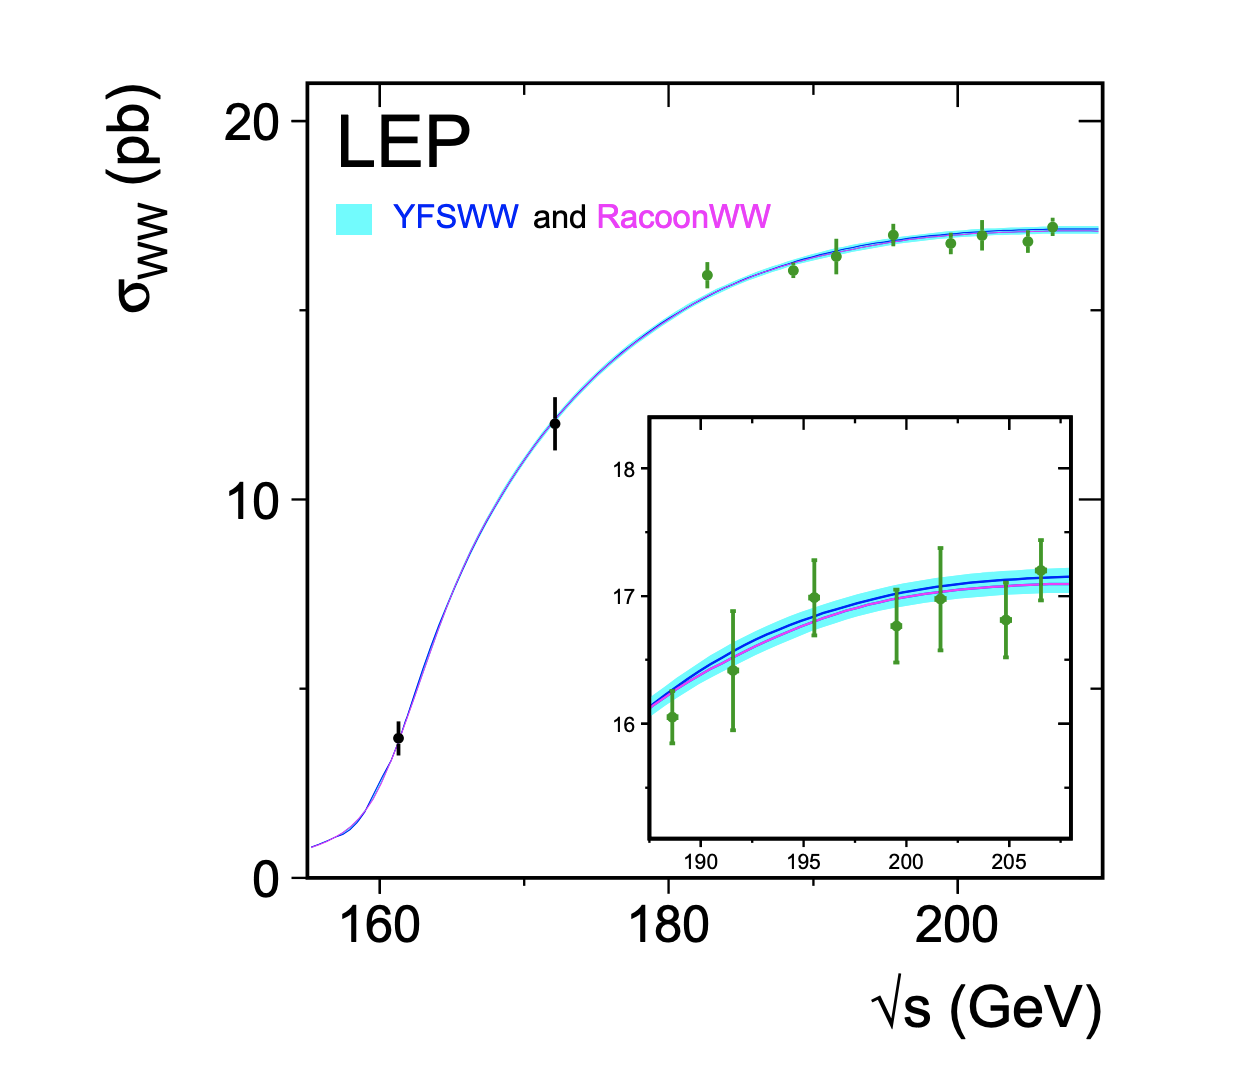
\includegraphics[width=0.49\textwidth]{chapters/RelatedWorks/sectionLU/figures/lep_ww.png}
    \caption{The LEP measurement of WW production cross-section. The measurement was a combine of the four LEP experiments, with a total 3~\fbinv  data. The WW production at LEP was mainly induced by exchanging neutrinos in the t-channel and quark annihilation to $Z/\gamma$  in the s-channel. The measured cross-section agreed with the theoretical calculation.}
    \label{fig:relatedWorks:lu:W:lepWWxs}
\end{figure}

Each experiment determined the leptonic \PW decay branching fractions from the WW cross-sections measurement, with and without the lepton universality assumption \cite{Schael:2013ita}. The hadronic branching fraction was determined from the leptonic ones based on the unitarity. When combining the four experiments, the theoretical uncertainties of signal and background, as well as the theoretical uncertainties of the luminosity, were treated as correlated; in contrast, the experimental uncertainties on the luminosity, detector effects, and MC statistics are treated as uncorrelated. The details of the $B(W\to l \nu)$ results and the correlations, in individual experiment and after being combined, are summarized in Table~\ref{tab:relatedWorks:lu:W:lep} and in Figure~\ref{fig:relatedWorks:lu:W:lep}. A clear excess of the lepton universality was observed in the result. While the branching fractions to electron and muon agree well with each other, the branching fraction to tau is significantly larger than the average of the branching fraction to electron and muon. Assuming only partial lepton universality, the ratio between the $B(W\to \tau \nu)$ and the average of $B(W\to e \nu)$ and $B(W\to \mu \nu)$ were reported as \cite{Schael:2013ita} $1.066 \pm 0.025$, showing a 2.6 standard deviation from the lepton universality.


% LEP result plot
\begin{figure}[ht]
    \centering
    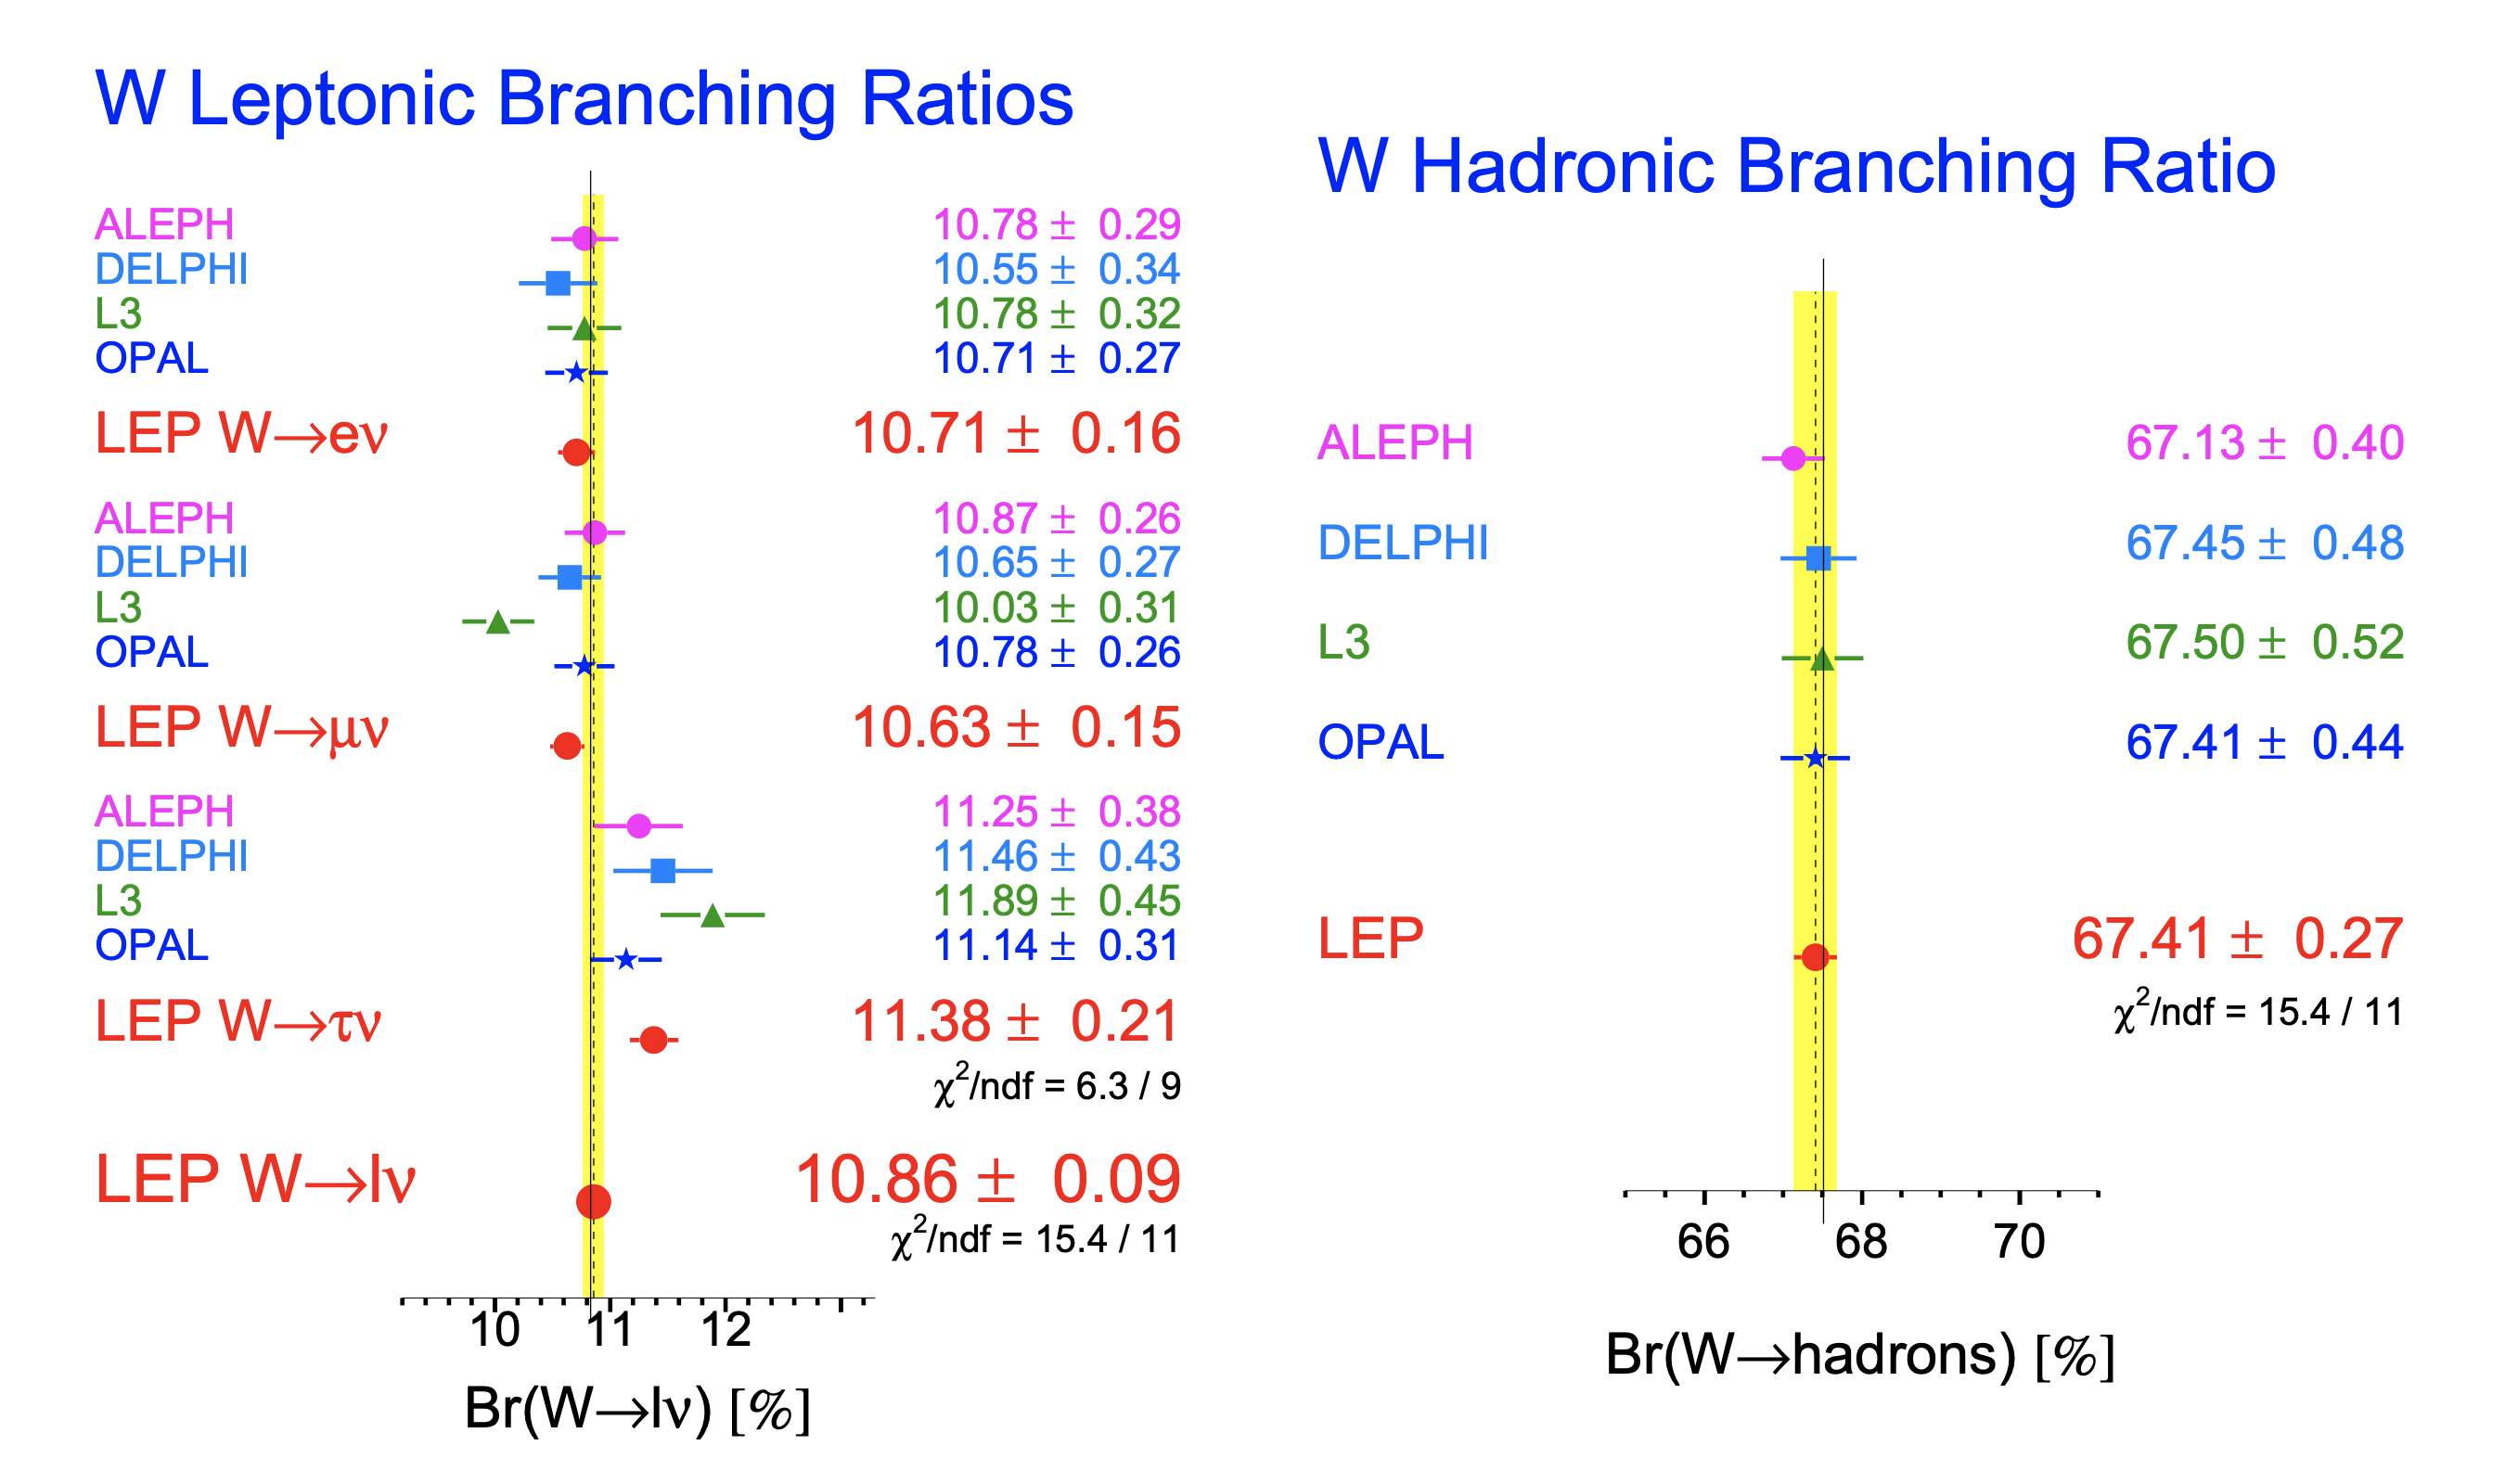
\includegraphics[width=0.99\textwidth]{chapters/RelatedWorks/sectionLU/figures/lepResult.png}
    \caption{\PW leptonic and hadronic branching fractions from the four LEP experiments. In the combined result, $B(W\to \tau \nu)$  is 2.6 $\sigma$ larger than the average of $B(W\to e \nu)$ and $B(W\to \mu \nu)$ \cite{Schael:2013ita}. }
    \label{fig:relatedWorks:lu:W:lep}
\end{figure}


% LEP result table
\begin{table}[!ht]
    \setlength{\tabcolsep}{.5 em}
    \renewcommand{\arraystretch}{1.5}
    \centering
    \caption{Three individual leptonic branching fractions from the four LEP experiments and the combined result \cite{Schael:2013ita}.}
    % \resizebox{\textwidth}{!}{
    \begin{tabular}{ |c| c  c | } 
         %  LEP ALEPH
         \hline
         \multicolumn{3}{|c|}{ALEPH \cite{Heister:2004wr}} \\
         \hline
         \BWe    & 10.78 $\pm$ 0.27 (stat) $\pm$ 0.10 (syst) & 
         \multirow{3}{*}{
            \begin{footnotesize}
            $\begin{bmatrix}
                +1.000 &-0.009 &-0.332 \\ 
                -0.009 &+1.000 &-0.268 \\
                -0.332 &-0.268 &+1.000 
            \end{bmatrix}$ 
            \end{footnotesize} 
         } \\
         \BWm    & 10.87 $\pm$ 0.25 (stat) $\pm$ 0.08 (syst) & \\ 
         \BWt    & 11.25 $\pm$ 0.32 (stat) $\pm$ 0.20 (syst) & \\
         \hline
         \multicolumn{3}{c}{} \\
         
         
         %  LEP DELPHI
         \hline
         \multicolumn{3}{|c|}{DELPHI \cite{Abdallah:2003zm}} \\
         \hline
         \BWe    & 10.55 $\pm$ 0.31 (stat) $\pm$ 0.14 (syst) & 
         \multirow{3}{*}{
            \begin{footnotesize}
            $\begin{bmatrix}
                +1.000 &+0.030 &-0.340 \\ 
                +0.030 &+1.000 &-0.170 \\
                -0.340 &-0.170 &+1.000 
            \end{bmatrix}$ 
            \end{footnotesize} 
         } \\
         \BWm    & 10.65 $\pm$ 0.26 (stat) $\pm$ 0.08 (syst) & \\ 
         \BWt    & 11.46 $\pm$ 0.39 (stat) $\pm$ 0.19 (syst) & \\
         \hline
         \multicolumn{3}{c}{} \\
         
         
         %  LEP L3
         \hline
         \multicolumn{3}{|c|}{L3 \cite{Achard:2004zw}} \\
         \hline
         \BWe    & 10.78 $\pm$ 0.29 (stat) $\pm$ 0.13 (syst) & 
         \multirow{3}{*}{
            \begin{footnotesize}
            $\begin{bmatrix}
                +1.000 &+0.136 &-0.201 \\ 
                +0.136 &+1.000 &-0.122 \\
                -0.201 &-0.122 &+1.000 
            \end{bmatrix}$ 
            \end{footnotesize} 
         } \\
         \BWm    & 10.03 $\pm$ 0.29 (stat) $\pm$ 0.12 (syst) & \\ 
         \BWt    & 11.89 $\pm$ 0.40 (stat) $\pm$ 0.20 (syst) & \\
         \hline
         
         \multicolumn{3}{c}{} \\
         
         %  LEP OPAL
         \hline
         \multicolumn{3}{|c|}{OPAL \cite{Abbiendi:2007rs}} \\
         \hline
         \BWe    & 10.71 $\pm$ 0.25 (stat) $\pm$ 0.11 (syst) & 
         \multirow{3}{*}{
            \begin{footnotesize}
            $\begin{bmatrix}
                +1.000 &+0.135 &-0.303 \\ 
                +0.135 &+1.000 &-0.230 \\
                -0.303 &-0.230 &+1.000 
            \end{bmatrix}$ 
            \end{footnotesize} 
         } \\
         \BWm    & 10.78 $\pm$ 0.24 (stat) $\pm$ 0.10 (syst) & \\ 
         \BWt    & 11.14 $\pm$ 0.31 (stat) $\pm$ 0.17 (syst) & \\
         \hline
         
         \multicolumn{3}{c}{} \\
         %  LEP Average
         \hline
         \multicolumn{3}{|c|}{LEP Average \cite{Schael:2013ita}} \\
         \hline
         \BWe    & 10.71 $\pm$ 0.14 (stat) $\pm$ 0.07 (syst) & 
         \multirow{3}{*}{
            \begin{footnotesize}
            $\begin{bmatrix}
                +1.000 &+0.136 &-0.201 \\ 
                +0.136 &+1.000 &-0.122 \\
                -0.201 &-0.122 &+1.000 
            \end{bmatrix}$ 
            \end{footnotesize} 
         } \\
         \BWm    & 10.63 $\pm$ 0.13 (stat) $\pm$ 0.07 (syst) & \\ 
         \BWt    & 11.38 $\pm$ 0.17 (stat) $\pm$ 0.11 (syst) & \\
         \hline
        %  *$Br(W\to \mu  \nu)/ Br(W\to e \nu)$ & 0.993  $\pm$ 0.019 & 
        %  \multirow{3}{*}{
        %     \begin{footnotesize}
        %     $\begin{bmatrix}
        %         +1.000 &+0.440 &-0.314 \\ 
        %         +0.440 &+1.000 &+0.714 \\
        %         -0.314 &+0.714 &+1.000 
        %     \end{bmatrix}$ 
        %     \end{footnotesize} 
        %  } \\
        %  *$Br(W\to \tau \nu)/ Br(W\to e \nu)$ & 1.063  $\pm$ 0.027 & \\
        %  *$Br(W\to \tau \nu)/ Br(W\to\mu\nu)$ & 1.070  $\pm$ 0.026 &  \\
         
        %  \hline
    \end{tabular}
    % }
    \label{tab:relatedWorks:lu:W:lep}
\end{table}


% \subsubsubsection{LHC Experiments}

\FloatBarrier
\underline{LHC}

During the LHC run~1 at a center-of-mass energy of 7 TeV and 8 TeV, the lepton universality test in the EW sector was studied in the electron and muon channel with W+jets events. Two such measurements were published by the ATLAS and LHCb. ATLAS measured the $\sigma_W \times B(W \to e \nu)$ and $\sigma_W \times B(W \to \mu \nu)$ \cite{Aaboud:2016btc} with 7 TeV proton-proton collision data with 4.6~\fbinv collected in 2011. The events in the electron and muon channel were triggered with the single-lepton trigger and selected with several lepton isolation and identification cut, as well as the met cut. The ratio between muon and electron was determined as $\frac{ B(W  \to \mu \nu) }{ B(W \to e \nu)} = 1.003\pm 0.010$. LHCb measured the $\sigma_W \times B(W \to e \nu)$ \cite{Aaij:2016qqz} and $\sigma_W \times B(W \to \mu \nu)$ \cite{Aaij:2015zlq} in two analysis with 8 TeV data corresponding to 2~\fbinv integrated luminosity. The events were also triggered with the single-lepton, and the selections required on lepton quality and met. To test universality between the electron and muon channel, the second analysis \cite{Aaij:2016qqz} compared the electron channel with the muon channel published in the first analysis \cite{Aaij:2015zlq}, taking into account the experimental correlations. The comparison included both the total cross-section and the differential cross-section with respect to pseudorapidity. The differential cross-section agreed well in the electron and muon channel. The ratio of the two total cross-section led to $\frac{ B(W  \to \mu \nu) }{ B(W \to e \nu)}  = 0.980 \pm 0.018 $.


During the LHC Run-II at a unprecedentedly high center-of-mass energy of 13~\TeV, \PW bosons from the \ttbar events are treated as the major signal in the LU test for the first time, thanks to the high \ttbar cross-section at 13~\TeV. ATLAS~\cite{Aad:2020ayz} measured the ratio between W to tau and W to muon branching fraction $B(W  \to \tau \nu) / B(W \to \mu \nu) $ using the LHC run~2 data from 2016-2018 at 13 TeV corresponding to 139~\fbinv. The analysis selects \ttbar events with a single-muon trigger and applies additional requirements on muon quality, jet multiplicity, and b-tag multiplicity for a \ttbar-enriched region. Tau is probed with tau's muonic decay, which is about 17\% of the total tau decay width. The key technique of this ATLAS measurement is fitting to the vertex displacement of the selected muon to discriminate $W \to \mu$ and $W \to \tau \to \mu$. Probing tau with muonic decay helps cancel the systematical uncertainties related to the muon reconstruction. Also, the systematics concerning hadronic tau reconstruction is avoided. The limitation of this approach is that only the $B(W  \to \tau \nu) / B(W \to \mu \nu) $ ratio is measured but the three individual leptonic branching fractions are not. The reported result of the $\tau / \mu $ branching ratio is

$$ \frac{ B(W  \to \tau \nu) }{ B(W \to \mu \nu)}  = 0.992 \pm 0.013 \text{ (ATLAS) }$$





\subsubsection{Test with Meson Decay}
\label{sec:relatedWorks:lu:meson}

% meson decay table
\begin{table}[ht]
    \setlength{\tabcolsep}{.5 em}
    \renewcommand{\arraystretch}{1.5}
    \centering
    \caption{SM prediction and the experimental measurements of the leptonic or semi-leptonic branching ratios of the pseudoscalar mesons. \cite{Bifani:2018zmi} }
    \resizebox{\textwidth}{!}{
    \begin{tabular}{|c|c|c|c|}
        \hline
         & SM Prediction & World Average & Included measurements \\
        \hline
        % pi
        $R^\pi_{e/\mu} \; [10^{-4}]$ &  1.2352 $\pm$ 0.0001 \cite{Cirigliano:2007xi} & 1.2327 $\pm$ 0.0023  & 
            \tiny{ TRIUMF \cite{Numao:1992ve, Britton:1992pg}, PiENu \cite{Aguilar-Arevalo:2015cdf}, BGO-OD \cite{Czapek:1993kc}} \\
        % K
        $R^K_{e/\mu} \; [10^{-5}]$ &  2.477  $\pm$ 0.001 \cite{Cirigliano:2007xi} & 2.488  $\pm$ 0.009 & 
            \tiny{NA62 \cite{Lazzeroni:2012cx}, KLOE \cite{Ambrosino:2009aa} }\\
        % D_s
        $R^{D_s}_{\tau/\mu} $ &  9.76 $\pm$ 0.10 \cite{Dobrescu:2008er} & 9.95 $\pm$ 0.61  & 
            \tiny{ HFLAV \cite{Amhis:2016xyh} ave of CLEO, BASIII, BELLE, BABAR} \\
        
        \hline
        % B D
        $R^{B}_{D, \tau/l} $ &  0.299  $\pm$ 0.003  \cite{Bifani:2018zmi} & 0.340  $\pm$ 0.030 & 
            \tiny{BABAR \cite{Lees:2012xj, Lees:2013uzd}, Belle \cite{Huschle:2015rga} }\\
            
        % B D*
        $R^{B}_{D*, \tau/l} $ &  0.258  $\pm$ 0.005 \cite{Bifani:2018zmi} & 0.295  $\pm$ 0.014 & 
            \tiny{BABAR \cite{Lees:2012xj, Lees:2013uzd}, Belle \cite{Huschle:2015rga, Sato:2016svk, Hirose:2016wfn}, LHCb\cite{Aaij:2015yra,Aaij:2017uff, Aaij:2017deq} }\\
            
        \hline
    \end{tabular}}
    \label{tab:relatedWorks:lu:meson:ratio}
\end{table}

The charged weak current decay of mesons also provides tests of LU.  The most stringent constraints come from the study of leptonic decay of the charged pions or kaons, which are helicity suppressed in the SM.  The level of helicity suppression depends on the mass of the outcoming lepton. Pions and kaons can decay into electrons and muons, but not taus which are heavier than $\pi, K$. The ratio between the electronic and muonic branching fractions $R^\pi_{e/\mu},R^K_{e/\mu}$ are measured in the $\pi$ factories \cite{Numao:1992ve, Britton:1992pg, Aguilar-Arevalo:2015cdf, Czapek:1993kc} and $K$ factories \cite{Lazzeroni:2012cx, Ambrosino:2009aa} listed in Table~\ref{tab:relatedWorks:lu:meson:ratio}. The ratios are compared to the SM prediction with LU. For D meson, tauonic decay is possible, and the ratio between tauonic and muonic branching fraction $R^D_{\tau/\mu}$ is measured in the charm factories including CLEO, BASIII, Belle, and BaBar. Table~\ref{tab:relatedWorks:lu:meson:ratio} shows these experimental measurements and the comparison to the SM theoretical calculations. The experimental results of purely leptonic decay of the light and charm pseudoscalar mesons agree well with the SM theoretical prediction. 

Additionally, the tests of LU can be performed by comparing semileptonic charged weak decays, such as $D\to K l\nu$. Heavy Flavor Averaging Group (HGLAV) provides a summary of the LU test using the semileptonic charged weak decay of the D meson and the B meson \cite{Amhis:2019ckw}. An anomaly is observed in the $B\to D^{(*)} l\nu$ semileptonic decay in the tau channel versus the electron and muon channel. $R^{B}_{D^{(*)}, \tau/l}$ is measured in the Belle \cite{Huschle:2015rga, Sato:2016svk, Hirose:2016wfn}, BaBar  \cite{Lees:2012xj, Lees:2013uzd} and LHCb \cite{Aaij:2015yra,Aaij:2017uff, Aaij:2017deq}, where ratio is defined as $R^{B}_{D, \tau/l} = \frac{Br(B\to D\tau \nu)}{Br(B\to Dl \nu)}$ and $R^{B}_{D^*, \tau/l} = \frac{Br(B\to D^*\tau \nu)}{Br(B\to D^*l \nu)}$ where $l=e,\mu$ . The experimental results are listed in Table~\ref{tab:relatedWorks:lu:meson:ratio}. Figure~\ref{fig:relatedWorks:lu:meson:bMesonDecay} illustrates this anomaly of the B meson semileptonic decay. The world average of Belle, BaBar and LHCb is about 4 sigma deviated from the SM theoretical prediction.

% However, these tests require knowledge of the ratio of the form factors of the scalar and vector meson, f0/f+, with very high accuracy to be competitive with the leptonic decays, where the main hadronic input (meson decay constants) drops out of the LU ratios. 



% B meson decay plot
\begin{figure}[ht]
    \centering
    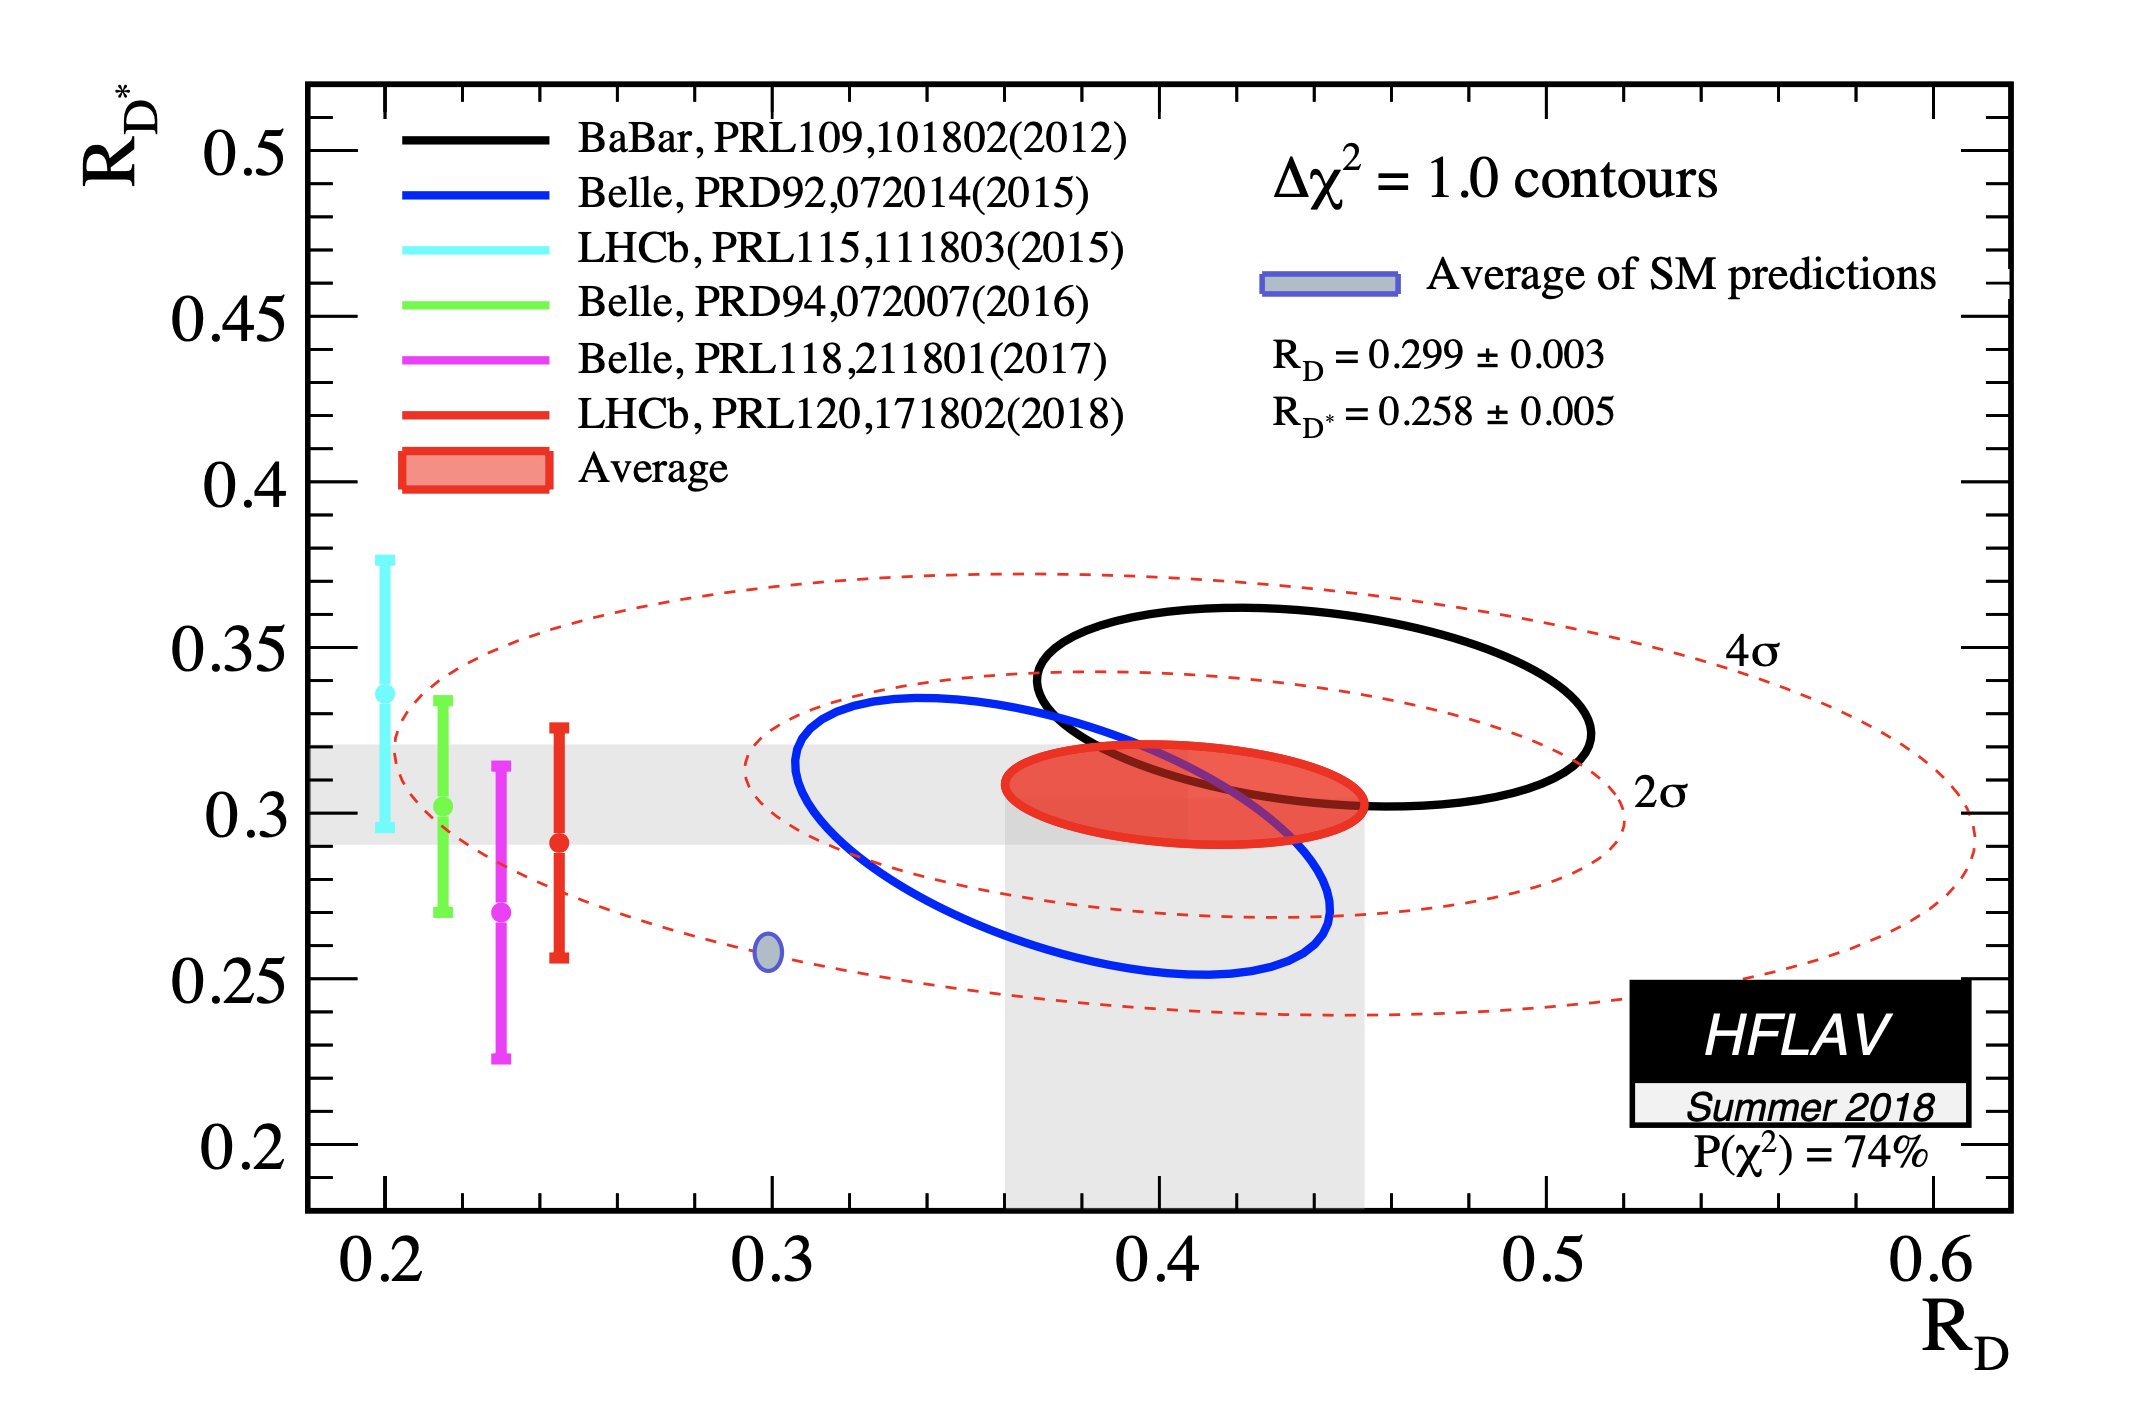
\includegraphics[ width = 0.7 \textwidth ]{chapters/RelatedWorks/sectionLU/figures/bmeson.png}
    \caption{ Anomaly of lepton universality in the semi-leptonic decay of B meson \cite{Amhis:2019ckw}. SM prediction and the world average of $R^{B}_{D, \tau/l}$  and $R^{B}_{D^*, \tau/l}$  shows a 4 sigma deviation.}
    \label{fig:relatedWorks:lu:meson:bMesonDecay}
\end{figure}




\subsubsection{Test with Tau Decay}
\label{sec:relatedWorks:lu:lepton}

The LU of charged weak current can also be tested by the tau precision measurements \cite{Pich:2013lsa,Amhis:2019ckw}. In the SM, the only expected difference between the $\tau^- \to e^- \bar{\nu}_e \nu_\tau$  and $\tau^- \to \mu^- \bar{\nu}_\mu \nu_\tau$  decay is due to decay kinematic phase space due to the mass of the outcoming leptons. $g_\mu  / g_e $ can be obtained by precision measurement of the tau decay in the electron and muon channels. Similarly,  $g_\tau  / g_\mu $ can be obtained by precision measurement of electronic tau decay  $\tau^- \to e^- \bar{\nu}_e \nu_\tau$ and electronic muon decay  $\mu^- \to e^- \bar{\nu}_e \nu_\mu$.  The ratio of the charged weak boson couplings to the third and first family can be obtained from the measurements of the $\tau^- \to \mu^- \bar{\nu}_\mu \nu_\tau$  and $\mu^- \to e^- \bar{\nu}_e \nu_\mu$  branching fraction and the $\tau,\mu$ lifetimes.  These represent one of the most stringent experimental tests for LU in the EW sector. By global fit to the tau precision measurements, HFLAV~\cite{Amhis:2019ckw} determines the ratios of EW coupling constant among the three leptons as 

\begin{align*}
    g_\tau / g_\mu &= 1.0010 \pm 0.0014 \\
    g_\tau / g_e   &= 1.0029 \pm 0.0014 \\
    g_\mu  / g_e   &= 1.0018 \pm 0.0014 
\end{align*}





\subsection{Measurements of $V_{cs}$ }
\label{sec:relatedWorks:vcsMeasurements}

The CKM matrix originates from the Yukawa couplings in the SM Higgs sector. It represents the mixing between quarks' mass eigenstates and the flavor eigenstates. When physical quarks in their mass eigenstates participate in the weak interaction, they are projected to the flavor eigenstates by the corresponding element in the CKM matrix. More details about the CKM in the standard model are discussed in Appendix~\ref{sec:relatedWorks:qft:gws}. 

\begin{table}[ht]
    \centering
    \setlength{\tabcolsep}{1.5em}
    \renewcommand{\arraystretch}{1.5}
    \caption{The current experimental world average of the 9 elements in the CKM matrix in the PDG \cite{pdg2020}.  }
    \resizebox{\textwidth}{!}{
    \begin{tabular}{c|c|c }
        \hline
        $|V_{ud}|=0.97370 \pm 0.00014 $     & $|V_{us}|=0.2245 \pm 0.0008$      &  $|V_{ub}|=0.00382 \pm 0.00024$   \\ \hline
        $|V_{cd}|=0.221 \pm 0.004 $         & $|V_{cs}|=0.987 \pm 0.011$        &  $|V_{cb}|=0.0410 \pm 0.0014$     \\ \hline
        $|V_{td}|=0.0080 \pm 0.0003 $       & $|V_{ts}|=0.0388 \pm 0.0011$      &  $|V_{tb}|=1.013 \pm 0.030$       \\
        \hline
    \end{tabular}}
    \label{tab:relatedWorks:vcs:ckm}
\end{table}


The current experimental measurement of the 9 elements in the CKM matrix \cite{pdg2020} is shown in Table~\ref{tab:relatedWorks:vcs:ckm}. Among the 6 elements in the first two rows, $|V_{cs}|$ is measured with the least precision. The average of $|V_{cs}|$ measurements is shown in Figure~\ref{fig:relatedWorks:vcs:measurements}. Currently, there are two direct approaches to measure $|V_{cs}|$, using the D meson decay in the charm factories and using the on-shell $W\to c s$  with jet tagging in the collider experiments.

The best direct determination of $|V_{cs}|$ is from the semileptonic decay of $D$ and the leptonic decay of $D_s$ produced in the charm factory. For the results from the leptonic decay of $D_s$ meson, the branching fraction of $D_s^+ \to \mu^+ \nu$ and $D_s^+ \to \tau^+ \nu$ are both measured in the Belle \cite{Zupanc:2013byn}, CLEO \cite{Alexander:2009ux,Onyisi:2009th,Naik:2009tk}, BaBar \cite{delAmoSanchez:2010jg} and BESIII \cite{Ablikim:2016duz, Ablikim:2018jun}. Using the experimental value of mass and lifetime of $D_s$, as well as the lattice QCD calculation of the form factor $f_{D_s}$, $|V_{cs}|$ can be determined from the $D_s$ leptonic decay and yields a world average of $|V_{cs}|=0.992\pm 0.012$ \cite{Amhis:2019ckw}, where the dominating uncertainty is from the experimental error. For the results from the semileptonic decay of $D$ meson, the branching fraction of $D\to K l\nu$ is measured by CLEO-c \cite{Besson:2009uv}, Belle \cite{Widhalm:2006wz}, BaBar \cite{Aubert:2007wg} and BESIII \cite{Ablikim:2015ixa, Ablikim:2018evp}, which gives an average of $|V_{cs}|$ of $|V_{cs}|=0.939\pm 0.038$ \cite{Amhis:2019ckw} in the D meson decay. The dominant uncertainty is form the theoretical calculations of the D meson form factor with latice QCD. Combining the result from the $D$ and $D_s$ decay, the charm factories measures $|V_{cs}|=0.987\pm 0.011$ \cite{Amhis:2019ckw}. This is also the value considered as the world average by the PDG~\cite{pdg2020}.

The second direct measurement of $|V_{cs}|$ is from the on-shell $W\to c s$ decays in the collider experiments. This approach relies on jet tagging to identifies the jets originating from the c and s quarks, which is relatively difficult, especially in the hadron collider with a more complex hadron environment. Therefore, this approach is less explored compared with the $D/D_s$ approach. So far, the only published result based on the $W\to c s$  approach is from the DELPHI~\cite{Abreu:1998ap} in the LEP. DELPHI identified the charged mesons based on their ionization energy loss while traversing through the TPC tracking system. Since s and c jets tend to include energetic kaons, c and s jets were first tagged by the \pt and the particle id ($\pi$ or K) of the leading meson in the jet. Then the impact parameters of the tracks in the jet were considered to discriminate c jets against other quarks. The result from DELPHI were reported as $|V_{cs}|=0.94 ^{+0.32}_{-0.26}\pm 0.13$. 

% In Figure~\ref{fig:relatedWorks:vcs:measurements}, the indirect measurement of $|V_{cs}|$ is from the global fit by CKMFitter to all the measured CKM elements assuming the four SM parameters. 

In addition, LEP published one indirect result. LEP measures the $Br(W\to l \nu) = (10.83 \pm 0.07 \pm 0.07) \%$ \cite{Schael:2013ita}, based on which calculates the sum of all six CMK element in the first two rows as $\sum |V_{ij}|^2 = 2.002 \pm 0.027$. Since $|V_{cs}|$ is the least precisely measured element, LEP subtract other five elements from $|V_{ij}|^2 $ and produces an indirect measurement of $|V_{cs}|=0.969\pm 0.013$. With the latest CKM values for the other five element in the first two rows, repeating LEP's calculation gives $|V_{cs}|=0.972\pm 0.013$. This thesis measures the $Br(W\to l \nu)$. Therefore, the same calculation as LEP can be done for our result to get $|V_{cs}|$ from $Br(W\to l \nu)$.


 \begin{figure}
    \centering
%     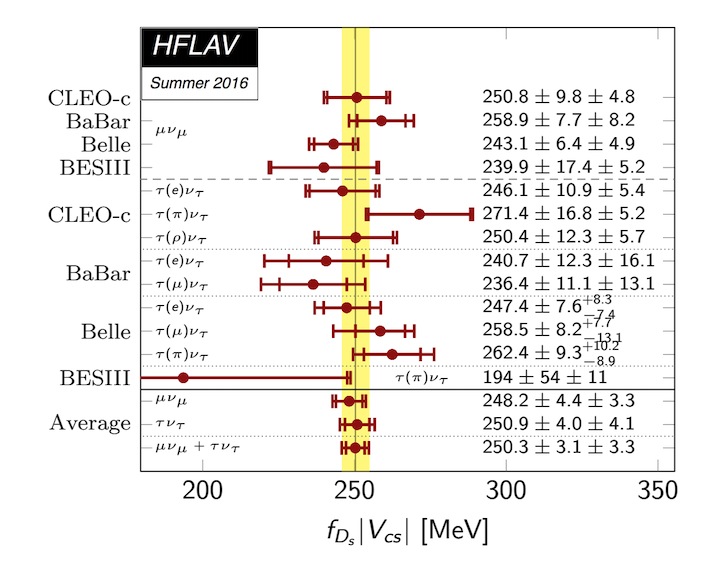
\includegraphics[width=0.45\textwidth]{vcs_meson_ds.png} \qquad
    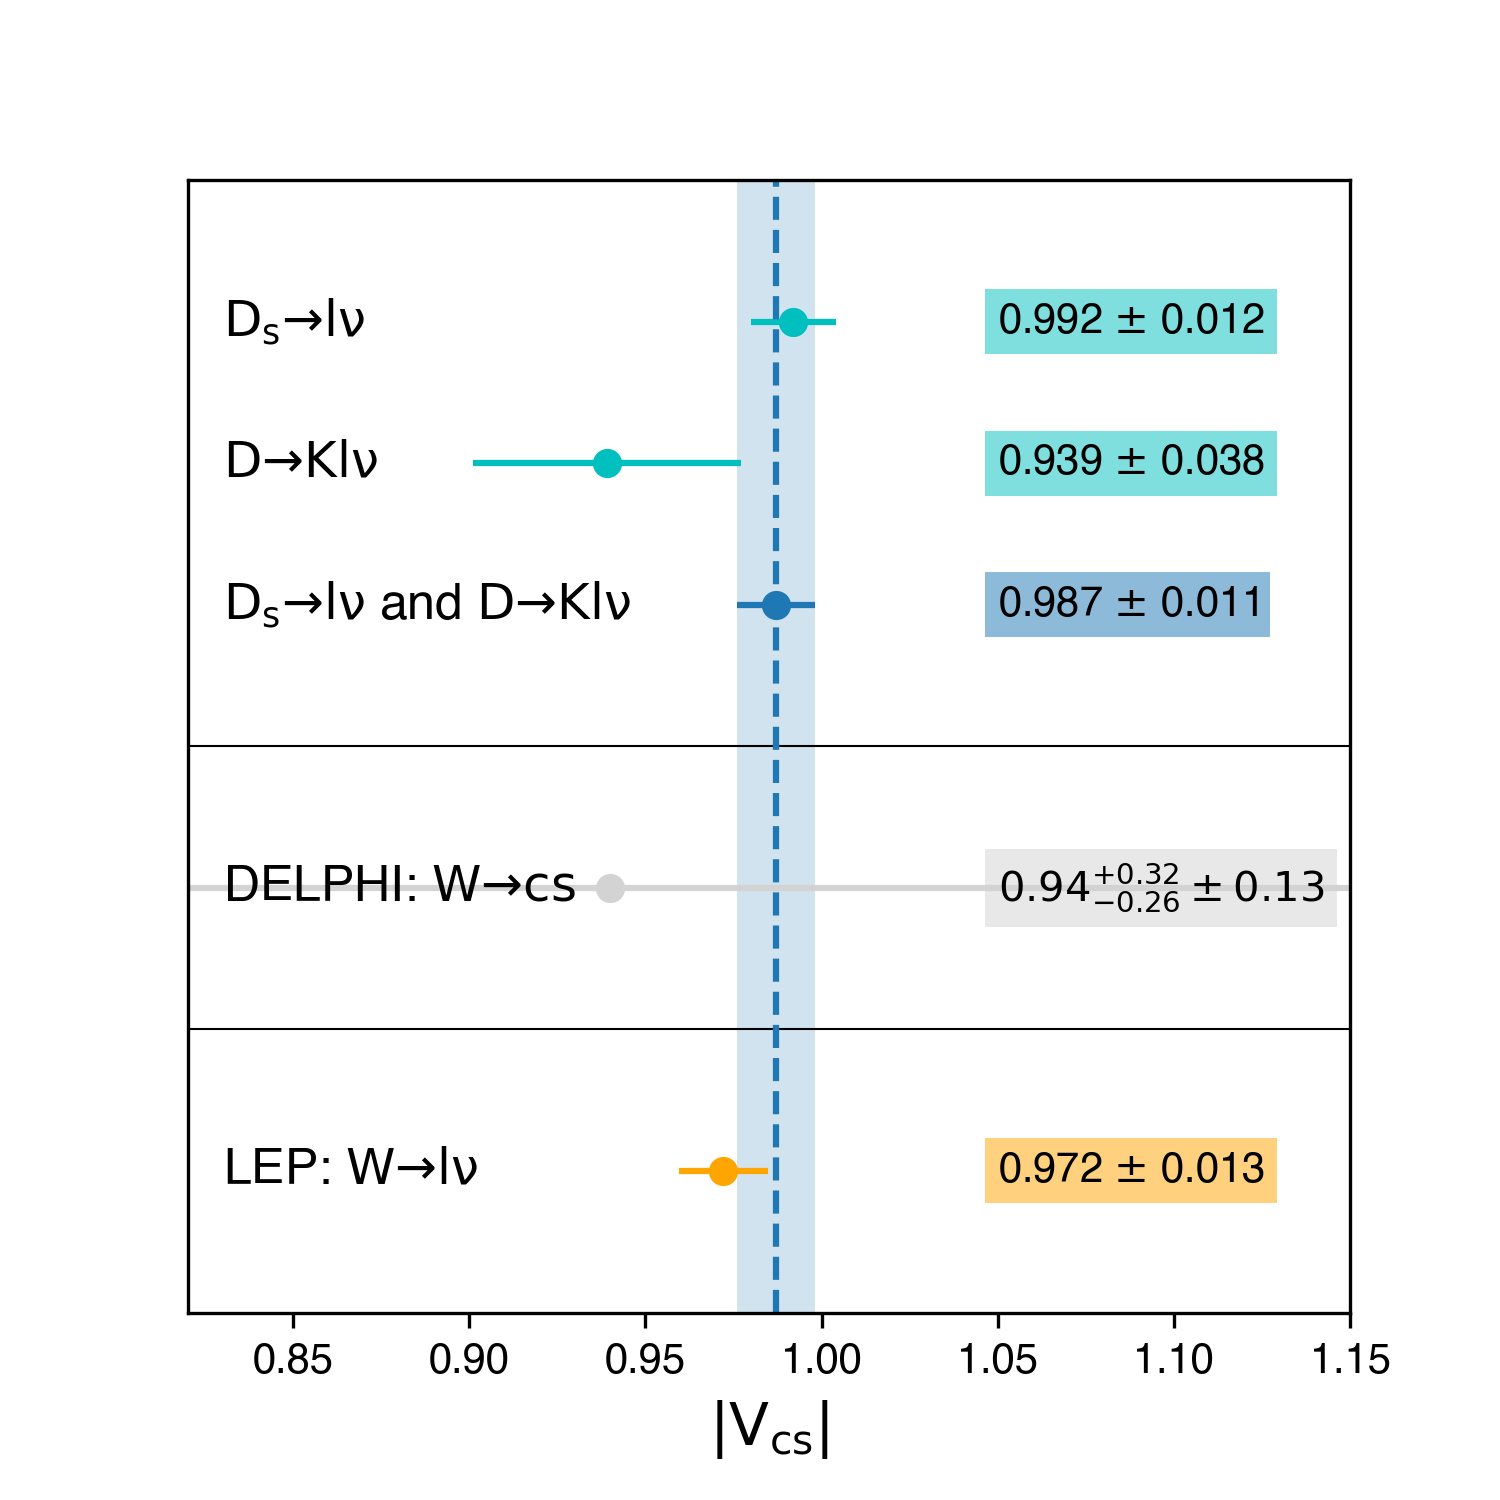
\includegraphics[width=0.6\textwidth]{chapters/RelatedWorks/sectionVcs/figures/vcs_world_average0.png}
    \caption{The $|V_{cs}|$ measurements~\cite{pdg2020}. The 2020 PDG average~\cite{pdg2020} combines the results from $D$ and $D_s$ decay.}
    \label{fig:relatedWorks:vcs:measurements}
\end{figure}





% \section{Measurements of $V_{cs}$ }

The CKM matrix originates from the Yukawa couplings in the SM Higgs sector. It represents the mixing between quarks' mass eigenstates and the flavor eigenstates. When physical quarks in their mass eigenstates participate in the weak interaction, they are projected to the flavor eigenstates by the corresponding element in the CKM matrix. More details about the CKM in the standard model are discussed in Section~\ref{sec:relatedWorks:qft:gws}. 

\begin{table}[ht]
    \centering
    \setlength{\tabcolsep}{1.5em}
    \renewcommand{\arraystretch}{1.5}
    \caption{The current experimental world average of the 9 elements in the CKM matrix in the PDG \cite{pdg2020}.  }
    \resizebox{\textwidth}{!}{
    \begin{tabular}{c|c|c }
        \hline
        $|V_{ud}|=0.97370 \pm 0.00014 $     & $|V_{us}|=0.2245 \pm 0.0008$      &  $|V_{ub}|=0.00382 \pm 0.00024$   \\ \hline
        $|V_{cd}|=0.221 \pm 0.004 $         & $|V_{cs}|=0.987 \pm 0.011$        &  $|V_{cb}|=0.0410 \pm 0.0014$     \\ \hline
        $|V_{td}|=0.0080 \pm 0.0003 $       & $|V_{ts}|=0.0388 \pm 0.0011$      &  $|V_{tb}|=1.013 \pm 0.030$       \\
        \hline
    \end{tabular}}
    \label{tab:relatedWorks:vcs:ckm}
\end{table}


The current experimental measurement of the 9 elements in the CKM matrix \cite{pdg2020} is shown in Table~\ref{tab:relatedWorks:vcs:ckm}. Among the 6 elements in the first two rows, $|V_{cs}|$ is measured with the least precision. The average of $|V_{cs}|$ measurements is shown in Figure~\ref{fig:relatedWorks:vcs:measurements}. Currently, there are two direct approaches to measure $|V_{cs}|$, using the D meson decay in the charm factories and using the on-shell $W\to c s$  with jet tagging in the collider experiments.

The best direct determination of $|V_{cs}|$ is from the semileptonic decay of $D$ and the leptonic decay of $D_s$ produced in the charm factory. For the results from the leptonic decay of $D_s$ meson, the branching fraction of $D_s^+ \to \mu^+ \nu$ and $D_s^+ \to \tau^+ \nu$ are both measured in the Belle \cite{Zupanc:2013byn}, CLEO \cite{Alexander:2009ux,Onyisi:2009th,Naik:2009tk}, BaBar \cite{delAmoSanchez:2010jg} and BESIII \cite{Ablikim:2016duz, Ablikim:2018jun}. Using the experimental value of mass and lifetime of $D_s$, as well as the lattice QCD calculation of the form factor $f_{D_s}$, $|V_{cs}|$ can be determined from the $D_s$ leptonic decay and yields a world average of $|V_{cs}|=0.992\pm 0.012$ \cite{Amhis:2019ckw}, where the dominating uncertainty is from the experimental error. For the results from the semileptonic decay of $D$ meson, the branching fraction of $D\to K l\nu$ is measured by CLEO-c \cite{Besson:2009uv}, Belle \cite{Widhalm:2006wz}, BaBar \cite{Aubert:2007wg} and BESIII \cite{Ablikim:2015ixa, Ablikim:2018evp}, which gives an average of $|V_{cs}|$ of $|V_{cs}|=0.939\pm 0.038$ \cite{Amhis:2019ckw} in the D meson decay. The dominant uncertainty is form the theoretical calculations of the D meson form factor with latice QCD. Combining the result from the $D$ and $D_s$ decay, the charm factories measures $|V_{cs}|=0.987\pm 0.011$ \cite{Amhis:2019ckw}.

The second direct measurement of $|V_{cs}|$ is from the on-shell $W\to c s$ decays in the collider experiments. This approach relies on jet tagging to identifies the jets originating from the c and s quarks, which is relatively difficult, especially in the hadron collider with a more complex hadron environment. Therefore, this approach is less explored compared with the $D/D_s$ approach. So far, the only published result based on the $W\to c s$  approach is from the DELPHI in the LEP, which reports $|V_{cs}|=0.94 ^{+0.32}_{-0.26}\pm 0.13$. \cite{Abreu:1998ap}

In Figure~\ref{fig:relatedWorks:vcs:measurements}, the indirect measurement of $|V_{cs}|$ is from the global fit by CKMFitter to all the measured CKM elements assuming the four SM parameters. In addition, LEP published another indirect result. LEP measures the $Br(W\to l \nu) = (10.83 \pm 0.07 \pm 0.07) \%$ \cite{Schael:2013ita}, based on which calculates the sum of all six CMK element in the first two rows as $\sum |V_{ij}|^2 = 2.002 \pm 0.027$. Since $|V_{cs}|$ is the least precisely measured element, LEP subtract other five elements from $|V_{ij}|^2 $ and produces an indirect measurement of $|V_{ij}|=0.969\pm 0.013$. This thesis measures the $Br(W\to l \nu) $ as well. Therefore, the same calculation as LEP can be done for our result to get $|V_{cs}|$ from $Br(W\to l \nu)$. The next part of this section covers about the steps of the such calculations.


 \begin{figure}
    \centering
%     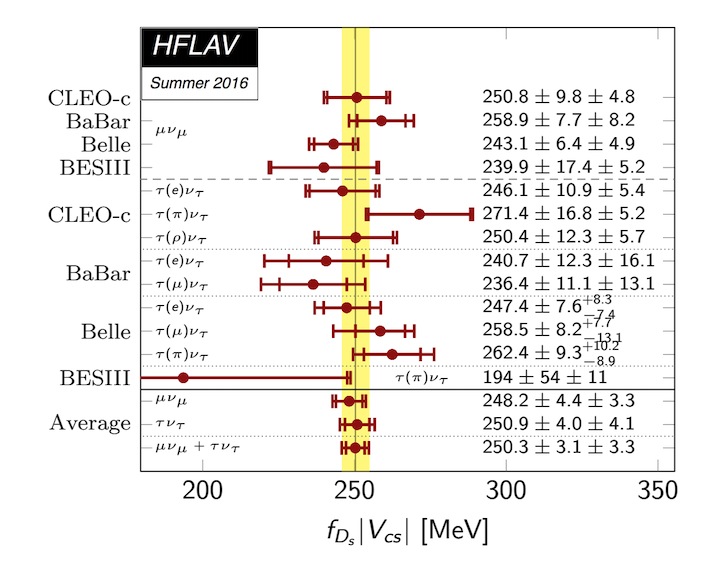
\includegraphics[width=0.45\textwidth]{vcs_meson_ds.png} \qquad
    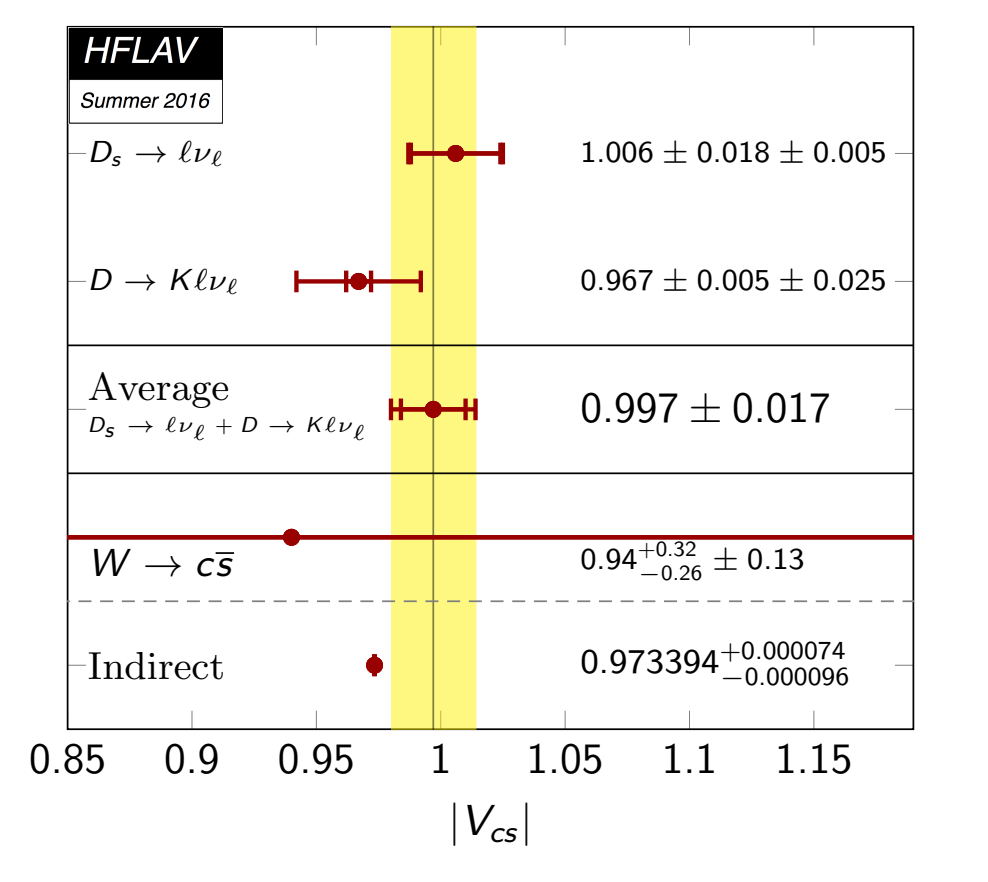
\includegraphics[width=0.6\textwidth]{chapters/RelatedWorks/sectionVcs/figures/vcs.png}
    \caption{The world average of $|V_{cs}|$ measurements. }
    \label{fig:relatedWorks:vcs:measurements}
\end{figure}
